\documentclass[fontsize=8pt,twoside=false,parskip=half,headings=small,numbers=withenddot,usegeometry=true,english]{scrartcl}

% Packages que conozco
\usepackage[T1]{fontenc} % Necesario para acceder a caracteres especiales
%\usepackage{lmodern} % Fuentes
\usepackage{upgreek} % Caracteres especiales (\uptau, etc.)
%\usepackage[utf8x]{inputenc} % IDEM
\usepackage[english]{babel} % Idioma principal del documento
\usepackage[table,usenames,dvipsnames]{xcolor} % Colores extra para las fuentes
\usepackage{graphicx} % Insertar imágenes
\usepackage{geometry} % Tamaño de Página y Márgenes
\usepackage{enumitem,pifont,textcomp} % Enumerar (letras, números, símbolos, etc.)
\usepackage{multicol} % Texto en columnas
\usepackage{titlesec} % Editar más fácilmente los colores de secciones, subseccinoes, etc.
\usepackage{empheq} % Attractive Boxed Equations
\usepackage[thinc]{esdiff} % Shorthand derivatives
\usepackage{subcaption} % Para poner figuras al lado de las otras
\usepackage{anyfontsize}
\usepackage{centernot}

% Configuración de algunos packages que conozco
\geometry{paper=legalpaper, landscape, left=6mm,right=6mm, top=6mm, bottom=4mm}

% Otros packages
%\usepackage{cmbright}
\usepackage[scaled=.90]{beramono}
\usepackage{tabulary}
\usepackage{booktabs}
\usepackage{microtype}
\usepackage{pdfpages}
\usepackage[autostyle=true]{csquotes}	
\usepackage{amsmath,amsthm, amssymb,nicefrac}
\usepackage{mathtools} % ???
\usepackage[sticky-per=true,per-mode=fraction]{siunitx}
\usepackage{float}

% Plots & Graphs
\usepackage{pgfplots}
	\usetikzlibrary{
		calc,
		patterns,
		positioning,
		arrows.meta,
		petri,
		positioning,
		calligraphy
	}
	\pgfplotsset{
		compat=1.17,
		samples=200,
		clip=false,
		1Quad/.style={
			axis x line=middle,
			axis y line=middle,
			legend pos=outer north east,
			axis line style={->},
			legend style={font=\tiny},
			label style={font=\tiny},
			tick label style={font=\tiny},
			xlabel style={at={(ticklabel* cs:1)},anchor=west,font=\tiny,},
			ylabel style={at={(ticklabel* cs:1)},anchor=west,font=\tiny,},
			%xlabel=$X$,
			%ylabel=$Y$
			},
		4Quad/.style={
			axis x line=middle,
			axis y line=middle,
			legend pos=outer north east,
			axis line style={->},
			legend style={font=\tiny},
			label style={font=\tiny},
			tick label style={font=\tiny},
			xlabel style={at={(ticklabel* cs:1)},anchor=west,font=\tiny,},
			ylabel style={at={(ticklabel* cs:1)},anchor=west,font=\tiny,}
			},
	}
	\tikzset{
		>=stealth
	}
\usetikzlibrary{math, angles, quotes, arrows.meta}

% Configuración que conozco
\setlist{noitemsep,itemindent=0pt,leftmargin=1.8em,nosep}
\setlist[itemize]{label*=\ding{223}}

% Otra Configuración
\arrayrulecolor{black}
\pagestyle{empty}
\abovedisplayskip=1pt\belowdisplayskip=0pt\abovedisplayshortskip=0pt\belowdisplayshortskip=0pt

% Bibliography (here for listings only)
\usepackage[backend=biber,style=verbose]{biblatex}

% Boxes
\providecommand{\titlebox}[1]{
	\fboxsep0.5em\hspace{-2.0\fboxsep}
	\fcolorbox{BrickRed}{BrickRed}{\parbox{\columnwidth}{\raggedright #1}}
}

\providecommand{\subtitlebox}[1]{
	\fboxsep0.5em\hspace{-2.0\fboxsep}
	\fcolorbox{lightgray}{lightgray}{\parbox{\columnwidth}{\raggedright #1}}
}

\providecommand{\sectionbox}[1]{\fboxsep0.5em\hspace*{-1.5\fboxsep}%
 \fcolorbox{gray}{gray!3}{%
 \parbox{\columnwidth}{%
 \raggedright #1}}}
 
\providecommand{\examplebox}[1]{\fboxsep0.5em\hspace*{-1.5\fboxsep}%
 \fcolorbox{gray}{Goldenrod!15!white!}{%
 \parbox{\columnwidth}{%
 \raggedright #1}}}

% Espacio entre párrafos
\setlength{\parskip}{2pt}
\renewcommand{\arraystretch}{1.5} % Tabular environments are properly displayed (haven't figured out why it doesn't work with 1)
\renewcommand{\baselinestretch}{1}

% Configuraciones de tablas
\setlength{\tabcolsep}{3pt}

% Fuente de secciones y subsecciones
%\setkomafont{disposition}{\color{Blue}} % Creo que esto es un comando total, para todo
\setkomafont{section}{\LARGE\bfseries\color{White}}
\setkomafont{subsection}{\large\bfseries\color{blue}}
\setkomafont{subsubsection}{\footnotesize\normalfont\bfseries\color{BrickRed}}

%\renewcommand*{\thesection}{\Alph{section}}
\setcounter{secnumdepth}{0}
\RedeclareSectionCommand[beforeskip=1pt, afterskip=5sp]{section}
\RedeclareSectionCommand[beforeskip=-2pt, afterskip=3sp]{subsection}
\RedeclareSectionCommand[beforeskip=-2pt, afterskip=3sp]{subsubsection}


% Path para las imágenes
\graphicspath{{img/}}

% Cprotect =====================================================================================
\usepackage{cprotect}
\def\AAAfoldernamecprotect{cpt_files} % Name of the folder in which .cpt files are stored

\makeatletter % This block is necessary implements the new destination of .cpt files
  \def\CPT@read@mbeg{%
  \stepcounter{CPT@WriteCount}%
  \edef\CPT@filename{./\AAAfoldernamecprotect/\jobname-\arabic{CPT@WriteCount}.cpt}%
  \expandafter\expandafter\expandafter\CPT@commandatend@toks
  \expandafter\expandafter\expandafter{%
    \expandafter\the
    \expandafter\CPT@commandatend@toks
    % Input a file:
    \expandafter{%
      \expandafter\protect
      \expandafter\input
      \CPT@filename
      \relax
    }%
  }%
  %\showthe\CPT@commandatend@toks%
  \begingroup%
  \makeallother%
  \def\CPT@preText{}%
  \let\CPT@postText\CPT@hat@hat@E@hat@hat@L%
  \let\CPT@begin\CPT@other@bgroup%
  \let\CPT@end\CPT@other@egroup%
  \CPT@readContent%
}%
\makeatother

% make boxes robust for verbatim
\let\oldsectionbox\sectionbox
\outer\def\sectionbox{\icprotect\oldsectionbox}

% Hyperref =====================================================================================
\usepackage{hyperref}
\renewcommand{\subsectionautorefname}{section}

\definecolor{darkblue}{RGB}{0, 82, 147}
\definecolor{annot}{RGB}{52, 135, 10}		
\hypersetup{
	pdfcreator={LaTeX2e},
	pdfborder=0 0 0,
	breaklinks=true,
	bookmarksopen=true,
	bookmarksnumbered=true,
	linkcolor=darkblue,
	urlcolor=darkblue,
	citecolor=darkblue,
	colorlinks=true,
	pdfauthor=Marion Lammarsch, 
	pdftitle=LaTeX Cheat Sheet,
	pdfcreator=LaTeX2e 
}
\urlstyle{sf}

% Source Code Listings ============
\usepackage{listings}
\lstset{
	backgroundcolor=\color{listinggray},
	basicstyle=\ttfamily\small,
	aboveskip={0.4\baselineskip},
	belowskip={0.4\baselineskip},
	literate={ä}{{\"a}}1 {ö}{{\"o}}1 {ü}{{\"u}}1 {Ä}{{\"A}}1 {Ö}{{\"O}}1 {Ü}{{\"u}}1 {ß}{{\ss}}1 {ô}{{\^o}}1	
}

\lstnewenvironment{mylatex} 
{\lstset{%
	backgroundcolor=\color{listinggray},
	%basicstyle=\ttfamily\small,
	tabsize=2,
	language={[LaTeX]TeX},
	%upquote=true,
	aboveskip={0.4\baselineskip},
	belowskip={0.4\baselineskip},
	abovecaptionskip={\baselineskip},
	belowcaptionskip={0\baselineskip},
	columns=fixed,
	showstringspaces=false,
	extendedchars=true,
	linewidth=.96\linewidth,
	xleftmargin=.04\linewidth,
	frameround=fttt,
	framexleftmargin={2pt},
	framexrightmargin={2pt},
	prebreak = \raisebox{0ex}[0ex][0ex]{\ensuremath{\hookleftarrow}},
	frame=single,
	showtabs=false,
	showspaces=false,
	showstringspaces=false,
	identifierstyle=\ttfamily,
	keywordstyle=\color{darkblue},
	commentstyle=\color[rgb]{0.133,0.545,0.133},
	stringstyle=\color[rgb]{0.8,  0.1,  0.1},
	morekeywords={part,chapter,subsection,subsubsection,paragraph,subparagraph,tableofcontents,%
		listoffigures,listoftables,printacronyms,ihead,ohead,clearscrheadings,clearmainofpairofpagestyles,%
		headmark,pagemark,maketitel,tr,varnothing,renewcommand,usepackage,includegraphics,graphicspath,%
		acsetup,DeclareAcroListStyle,DeclareAcronym,ac,Ac,definecolor,colorlet,textcolor,colorbox,%
		rowcolor,addbibresource,autocite,printbibliography,%	
		nexists,KOMAoptions,PassOptionsToPackage,thesection,thefigure,color,foreignlanguage},
	literate={ä}{{\"a}}1 {ö}{{\"o}}1 {ü}{{\"u}}1 {Ä}{{\"A}}1 {Ö}{{\"O}}1 {Ü}{{\"u}}1 {ß}{{\ss}}1 {ô}{{\^o}}1	
}}{}

\sloppy

% Macros y Nuevos comandos
\newcommand{\topline}{\vspace{2pt}{\color{Gray!80}\hrule}\vspace{3pt}}
\renewcommand{\qedsymbol}{$\!\! \blacksquare$}
\pgfplotsset{hide scale/.style={ /pgfplots/xtick scale label code/.code={}, 
								 /pgfplots/ytick scale label code/.code={}}
}
\newcommand{\bcentering}[1]{\par\vspace{1.5mm}{\centering \boxed{#1}\par}\vspace{1.5mm}}
\newcommand{\centerexpr}[1]{\par\vspace{1.25mm}{\centering #1\par}\vspace{1.25mm}}
\newcommand{\then}{\textcolor{blue}{\enspace\Rightarrow\enspace}}
\newcommand{\AND}{\textcolor{blue!70!black}{\;\,\land\;\,}}
\newcommand{\OR}{\textcolor{blue!70!black}{\;\,\lor\;\,}}
\newcommand{\ldraw}{black}
\newcommand{\Blue}[1]{\textcolor{blue}{#1}}
\newcommand{\Red}[1]{\textcolor{red}{#1}}
\newcommand{\Green}[1]{\textcolor{green!65!black}{#1}}

% Tikz Custom Figures
\tikzset{pics/bar/.style 2 args={code={ \fill (-.1,0) rectangle (.1,#1) (0,#1) node[above,scale=1/2]{$#2$}; }}}

% Distancia antes y después de cada {figure}
\setlength{\intextsep}{5pt plus 2pt minus 2pt}

% Corregir el problem de \implies y la fuente Revx Neue Demo ==================
\usepackage{lmodern}
\makeatletter
% Load the OT1 definitions for lmodern
\input{ot1lmr.fd}
% Change the definition for \OT1/lmr/m/n/<size>
\DeclareFontShape{OT1}{lmr}{m}{n}%
  {<-5.5>    rm-lmr5  <5.5-6.5> rm-lmr6
   <6.5-7.5> rm-lmr7  <7.5-8.5> rm-lmr8
   <8.5-9.5> rm-lmr9  <9.5->    rm-lmr10
  }{}
\makeatother
\usepackage{fontspec}
\setmainfont{Revx Neue Demo}
% ==============================================================================

% DOCUMENT_BEGINS ====================================================================================
\begin{document}

% FIRST 4 COLS
\begin{multicols*}{4}

\parbox{\columnwidth}{\centering\Huge\color{Black}\textbf{Probability \strut}}\scriptsize

\titlebox{\section{Probability Models and Axioms}}

\sectionbox{\subsubsection{Sample Space}\topline
Let the sample space $\Omega=\{\omega_1, \dots, \omega_n\}$ be the set of  all possible outcomes of an experiment or random trial. 
Let $\omega_i \in \Omega$ be a particular sample point or outcome.\\
\vspace{1.25mm}
In order to be a sample space, the set $\{\omega_1, \dots, \omega_n\}$ must meet certain conditions:
\begin{figure}[H]
	\begin{minipage}{1.75cm}
		\centering
		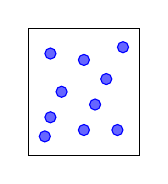
\begin{tikzpicture}
			\begin{axis}[
				hide axis,       % hide the axis
				xmin=0, xmax=1,  % set the x limits
				ymin=0, ymax=1,  % set the y limits
				clip=false,      % prevent clipping
				width=3cm,      % width of the plot
				height=3.2cm,     % height of the plot
			]
		
			% scatter plot of 10 specified points
			\addplot [
				only marks, 
				mark=*, 
				mark size=2pt,   % size of the dots
				draw=blue,         % color of the dot border
				fill=blue!60!white           % color of the dot interior
			] 
			coordinates {
				(0.15, 0.15)(0.2, 0.3)(0.3, 0.5)(0.5, 0.75)(0.5, 0.2)
				(0.6, 0.4)(0.7, 0.6)(0.8, 0.2)(0.85, 0.85)(0.2, 0.8)
			};
		
			% box
			\draw[line width=0.1mm] (axis cs:0,0) rectangle (axis cs:1,1);
			\end{axis}
		\end{tikzpicture}
		\end{minipage}%
		\begin{minipage}{6.5cm}
			\tiny{
				Outcomes must be \textbf{Mutually Exclusive},  i.e. if $\omega_i$ occurs, then no other $\omega_j$ will take place.
				$\forall i,j=1 \dots n , i \neq j.$
				\\ \vspace{0.1mm} \\
				Outcomes must be \textbf{Collectively Exhaustive}, i.e. on every experiment or trial, the outcome must be only $\omega_i \in \Omega.$
				\\ \vspace{0.1mm} \\
				The set must be at a \textbf{Right Granularity}, depending on what the experimenter is interested in.
				Irrelevant information must be removed from the set and the right abstraction must be chosen.
			}
		\end{minipage}
\end{figure}

}

\examplebox{\subsubsection{}
Consider the experiment of flipping a coin. Let $H$ and $T$ be the events heads and tails, respectively. Let $R$ be "it's raining" and $ \lnot R$ its negation.
\vspace{2mm}
\\
\begin{minipage}{4cm}
	\centering
		\tiny{$\Omega = \{H \land R, H \land \lnot R, T\}$} \\
		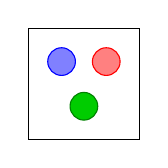
\begin{tikzpicture}
			\begin{axis}[hide axis, xmin=0, xmax=1, ymin=0, ymax=1, clip=false, width=3cm,height=3cm,]
				\draw[blue, fill=blue!50!white] (0.30, 0.70) circle (5pt);
				\draw[red, fill=red!50!white] (0.70, 0.70) circle (5pt);
				\draw[green!50!black, fill=green!80!black] (0.5, 0.30) circle (5pt);
				\draw[line width=0.1mm] (axis cs:0,0) rectangle (axis cs:1,1);
			\end{axis}
		\end{tikzpicture}
\end{minipage}%
\begin{minipage}{4cm}
	\centering
		\tiny{$\Omega = \{H \land R, T \land \lnot R, T\}$} \\
		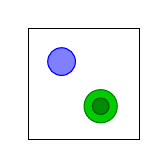
\begin{tikzpicture}
			\begin{axis}[hide axis, xmin=0, xmax=1, ymin=0, ymax=1, clip=false, width=3cm,height=3cm,]
				\draw[blue, fill=blue!50!white] (0.30, 0.70) circle (5pt);
				\draw[green!50!black, fill=green!80!black] (0.65, 0.30) circle (6pt);
				\draw[green!35!black, fill=green!55!black] (0.65, 0.30) circle (3pt);
				\draw[line width=0.1mm] (axis cs:0,0) rectangle (axis cs:1,1);
			\end{axis}
		\end{tikzpicture}
\end{minipage}%
\\ \vspace{2mm}
For the left case, we have a legitimate sample space. For the right case we have an outcome that it's included in another one, namely $\{T \land \lnot R\} \subset T$,
therefore the outcomes aren't mutually exclusive.
}

\sectionbox{\subsubsection{Discrete and Continuous, Finite and Infinite Sample Spaces}\topline
\begin{itemize}
	\item Discrete and Finite $\rightarrow$ Throwing 2 regular dice once:  $|\Omega|=6 \times 6=36$
	\item Discrete and Infinite $\rightarrow$ Guessing a natural number (?)
	\item Continuous and Infinite $\rightarrow$ The (x,y) coordinates of the landing of a dart 
\end{itemize}
}

\sectionbox{\subsubsection{Events}\topline
An event $A$ is a \textbf{subset} of the sample space $\Omega$, $\rightarrow A \subset \Omega $, i.e. an event $A$ is a set of outcomes itself. \\
Probability is assigned to events, $P(A)$. If events weren't defined in terms of subsets (sets), handling individual sample points in continuous sample spaces would be complicated. \\
}

\sectionbox{\subsubsection{Probability Axioms}\topline
Nonnegativity: $P(A) \geq 0$, $A$ is any event. \\
Normalization: $P(\Omega) = 1 $ (the event here is $\Omega$, since every set is subset of itself).\\
(Finite) Additivity (\textit{to be strengthened later}): $A \cap B = \emptyset \implies P(A \cup B) = P(A) + P(B)$\\
\vspace{2mm}
The last axiom is going to be refined later\\
These 3 axioms are sufficient to have a legitimate \textbf{probability model}.
}

\examplebox{\subsubsection{}
\begin{minipage}{1.75cm}
	\centering
		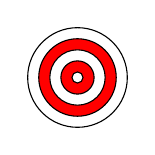
\begin{tikzpicture}
			\begin{axis}[hide axis, xmin=0, xmax=1, ymin=0, ymax=1, clip=false, width=2cm,height=2cm,]
			\addplot [only marks, mark=*, mark size=18pt, draw=black, fill=white] coordinates {(0.5, 0.5)};
			\addplot [only marks, mark=*, mark size=14pt, draw=black, fill=red] coordinates {(0.5, 0.5)};
			\addplot [only marks, mark=*, mark size=10pt, draw=black, fill=white] coordinates {(0.5, 0.5)};
			\addplot [only marks, mark=*, mark size=6pt, draw=black, fill=red] coordinates {(0.5, 0.5)};
			\addplot [only marks, mark=*, mark size=2pt, draw=black, fill=white] coordinates {(0.5, 0.5)};
			\end{axis}
		\end{tikzpicture}
\end{minipage}%
\begin{minipage}{6.5cm}
	Suppose the distribution of dart hits is uniform across the dart board, so the probability of hitting a point is $P(x, y) = \frac{1}{\text{Area}}$ over the region, and $0$ elsewhere.
	Since a single point has no area, we can express it as a region approaching zero, $R \to 0$.
	Therefore, the probability of \textbf{exactly hitting the center} of an infinite continuous space is:
	\\
		$P\big[(x, y) = (x_0, y_0)\big] = \lim\limits_{{R \to 0}} \iint_{R} f(x, y) \, dx \, dy = 0$
	\\
	since the integral over an infinitesimally small region $R$ will go to zero as $R$ goes to zero.
	But if we consider the event of hitting a region instead of a point, its probability is greater than zero. 
\end{minipage}%
}

\sectionbox{\subsubsection{Probability Model}\topline
Bertsekas \& Tsitsiklis definition: A Probabilistic Model is a mathematical description of an uncertain situation. It is composed of two main \textit{ingredients}: A Sample Space and
a Probility Law that specifies the likelihood of events.\\
\vspace{2mm}
\textbf{Probability Law:} The logic by which likelihood of outcomes is defined or assigned.\\
Consider the probability of hitting any subset of a $1\times 1$ square. $P(x,y) : 0 \leq x, y \leq 1 \rightarrow$ The probability of any particular subset of $\Omega$ is just its area (Uniform Probability).\\
\vspace{2mm}
For completeness (Sample Space, \textbf{Probability Space}, Probability Model):\\
-\url{https://stats.stackexchange.com/questions/199280/why-do-we-need-sigma-algebras-to-define-probability-spaces}\\
-\url{https://math.stackexchange.com/questions/2002416/defining-the-sigma-algebra-of-events-of-a-probability-space}\\
-\url{https://en.wikipedia.org/wiki/Probability_space}
}

\sectionbox{\subsubsection{Countable and Uncountable Sets}\topline
Segun Tsitsiklis, Discrete = Countable, alrededor del min 10:24, en el video 17, Lec. 1.
}

\sectionbox{\subsubsection{Consequences of the Axioms}\topline
By set theory definitions we have: \boxed{A \cup A^{c} = \Omega} \, and \,  \boxed{A \cap A^{c} = \emptyset}
\bcentering{P(A) \leq 1}
$A$ and $A^{c}$ are disjoint $\then P(A \cup A^{c}) = 1 = P(A) + P(A^{c}) \then P(A^{c}) = 1 - P(A)$,
and by \textit{nonnegativity} we get $P(A^{c}) \geq 0 \then P(A) \leq 1 \qed$
\bcentering{P(\emptyset) = 0}
Let $A = \Omega \then P(\Omega) + P(\Omega^{c}) = 1 \then 1 + \emptyset = 1  \then P(\emptyset) = 0 \qed$\\
\vspace{1.5mm}
Let $\Omega$ be a finite set and $A_{1},...,A_{n}$ be disjoint events, then:
\bcentering{P\left(\bigcup_{i=1}^{n}A_{i} \right) = \sum_{1}^{n} P(A_{i})}
$P(A \cup B \cup C)=P\left[(A \cup B) \cup C\right]$. From additivity, given that the events are disjoint, we have $(P(A) + P(B)) + P(C)$.
By induction we can extend this to $n$ disjoint sets $\qed$\\
\vspace{2mm}
Let $\{\omega_{1},...,\omega_{k}\}$ be a discrete, finite set of sample points, then:
\bcentering{P\big(\{\omega_{1},...,\omega_{k}\}\big) \then P\left(\,\bigcup_{j=1}^{k}\{\omega_{j}\} \right) \then \sum_{j=1}^{k}P\big(\{\omega_{j}\}\big)}
because $\{\omega_{1},\dots,\omega_{k}\}$, can be seen as the union of \textit{unit sets}, and since they are disjoint, additivity applies $\!\qed$.
Although, a simpler, non rigorous notation can be used: $\sum_{j=1}^{k}P(\omega_{j})$.
}

\examplebox{
Let $A, B, C$ be disjoint subsets of $\Omega$, then:\\
$P(A) + P(A^{c}) + P(B) \neq P(A \cup A^{c} \cup B) \rightarrow$ e.g. when: $A=\emptyset, B=\Omega$ \\
$P(A^{c}) + P(B) \nleq 1 \rightarrow$ e.g. when: $A=\emptyset, B=\Omega \then A^{c}=\Omega$ \\
Let $A, B, C$ be not necessarily disjoint subsets of $\Omega$, then:\\
$P[(A \cap B) \cup (C \cap A^{c})] \leq P(A \cup B \cup C) \rightarrow$ Since $(A \cap B), (C \cup A^{c})$ are its subsets.
}

\sectionbox{\subsubsection{More Consequences of the Axioms}\topline
Consider the condition $P(A \cap B) \geq 0, \then$ The events could be joint, therefore, more generally:\\
\vspace{1.5mm}
{\centering
	\begin{minipage}{1.75cm}
		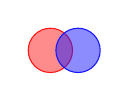
\begin{tikzpicture}
			\fill[draw=\ldraw, fill opacity=0.5, red!90!white] (0:0pt) circle (8pt);
			\fill[draw=\ldraw, fill opacity=0.5, blue!90!white] (0:10pt) circle (8pt);
		\end{tikzpicture}
	\end{minipage}%
	\begin{minipage}{4cm}
		\boxed{P(A \cup B) = P(A) + P(B) - P(A \cap B)}
	\end{minipage}
\\}
\vspace{1.5mm}
Which can be generalized to the \nameref{Inclusion-Exclusion Principle}:
\bcentering{P\left( \bigcup_{i=1}^{n} A_i\right) = -\sum_{k=1}^{n} (-1)^k \sum_{1 \leq i_{_1} < ... < i_{_k} \leq n} P \left( \, \bigcap_{j=1}^{k} A_{i_j} \right)}
From the above, the \textit{Union Bound} property follows: \boxed{P(A \cup B) \leq P(A) + P(B)}\\
\vspace{1.5mm}
Consider that $A$ is included in $B$, then:\\
\vspace{1.5mm}
{\centering
	\begin{minipage}{1.75cm}
		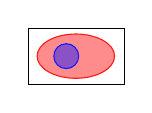
\begin{tikzpicture}
			\begin{axis}[hide axis, xmin=0, xmax=1, ymin=0, ymax=1, clip=false, width=2.8cm,height=2.3cm,]
				\fill[draw=\ldraw, fill opacity=0.5, red!90!white] (0.5,0.5) ellipse (14pt and 8pt);
				\fill[draw=\ldraw, fill opacity=0.5, blue!90!white] (0.4, 0.5) circle (4.5pt);
				\draw[line width=0.05mm] (axis cs:0,0) rectangle (axis cs:1,1);
			\end{axis}
		\end{tikzpicture}
	\end{minipage}%
	\begin{minipage}{3cm}
		\boxed{A \subset B \then P(A) \leq P(B)}
	\end{minipage}
\\}
\vspace{1.5mm}
since $B = A \cup (B \cap A^{c}) \then P(B) = P(A) + P(B \cap A^{c}) \geq P(A) \qed$ \\  
\vspace{1.5mm}

Consider 3 sets not necessarily disjoint, e.g.:\\
\vspace{1.5mm}
\begin{minipage}{2cm}
	\centering
	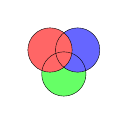
\begin{tikzpicture}
		\fill[draw=none, fill opacity=1, green!60!white] (0:0pt) circle (8pt);
		\fill[draw=none, fill opacity=1, blue!60!white] (60:10pt) circle (8pt);
		\fill[draw=none, fill opacity=1, red!60!white] (120:10pt) circle (8pt);
		\draw [draw=black, line width=0.05mm] (0:0pt) circle (8pt);
		\draw [draw=black, line width=0.05mm] (60:10pt) circle (8pt);
		\draw [draw=black, line width=0.05mm] (120:10pt) circle (8pt);
	\end{tikzpicture}
\end{minipage}%
\begin{minipage}{3cm}
	\boxed{P(A \cup B \cup C) =  \textcolor{red}{P(A)} + \textcolor{blue}{P(A^{c} \cap B)} + \textcolor{green!70!black}{P(A^{c} \cap B^{c} \cap C)}}
\end{minipage}
\\
\vspace{1.5mm}
Visually, we can check the boxed expression by the matching of the colors, and since the subsets are disjoint, additivity holds.  Notice the expression also applies to disjoint sets $\qed$
}

\sectionbox{\subsubsection{Pendiente...}\topline
- Discrete Probability Law \& Discrete Uniform Probability Law $\rightarrow$ Textbook. Añadir además un ejemplo similar al de la sección 14 \\
- Continuous Probability Law $\rightarrow$ \url{https://stats.stackexchange.com/questions/273382/how-can-the-probability-of-each-point-be-zero-in-continuous-random-variable}.
Incluir ademas algun ejemplo algo complejo como los de la seccion 16.
}

\sectionbox{\subsubsection{Countable Additivity Axiom}\topline
If $A_{1}, A_{2},...$ is an infinite \textbf{sequence} of disjoint events, then:
\bcentering{P(A_{1} \cup A_{2} \cup A_{3} \cup ...) = P(A_{1}) + P(A_{2}) + P(A_{3}) + ...}
The word sequence is important here since it's necessary to be able to arrange the events in some order.\\
\vspace{1.5mm}
Consider the following case:
The sample space consists of the unit square, the probability of a set/event is its area. Now, consider the probability of the whole $\Omega$ as the probability of the union
of all the $(x,y)$ points: $P(\Omega) = 1 = P\left(\bigcup \{(x,y)\}\right) = \sum P(\{x,y\}) = \sum 0 = 0$, we arrived to a seemingly contradiction because the elements of
the unit square (i.e. $(x,y)$ sets) can't be arranged in a sequence $\rightarrow$ The unit square is an uncountable set.\\
\vspace{1.5mm}
The proof for "countable/discrete = can be arranged in a sequence, uncountable/continous = can't be arranged in a sequence" is said to be found in Measure Theory.
}

\examplebox{
Ejemplo de sumatoria de serie infinita (ver ejercicios 18, 19, 20)
}

\examplebox{
Let the sample space be the set of all positive integers. Is it possible to have a “uniform" probability law, that is, a probability law that assigns the same 
probability $c$ to each positive integer?\\
\vspace{1.5mm}
Suppose that $c=0$. Then: $ 1=\mathbf{P}(\Omega )=\mathbf{P} (\{ 1\} \cup \{ 2\} \cup \{ 3\} ...)$, and by countable additivity this equals 
$\mathbf{P}(\{ 1\} )+\mathbf{P}(\{ 2\} )+\mathbf{P}(\{ 3\} )+... = \sum 0 = 0$, which is a contradiction.
\\ \vspace{1.5mm}
Suppose that $c>0$. Then, there exists an integer $k$ such that $kc>1$. By additivity, $P({1,2,...,k}) = kc > 1$. The answer is therefore \textbf{No}.
\\ \vspace{1.5mm}
\textbf{Important:} The question ask whether is possible to have a "uniform" probability law (each event has the same probability) from this discrete,
countable set, not whether \textbf{countable additivity} can be applied, which implies that a non-uniform probability law could be still applied.
}

\sectionbox{\subsubsection{Probability and Statistics Relationship}\topline
Insert the last figure from the PDF
}

\titlebox{\section{Conditioning and Independence}}
\subsection{Conditioning and Bayes' Rule}
\sectionbox{\subsubsection{Conditional Probability}\topline
Let $P(B)>0$, then the probability of $A$ given that $B$ has occurred is:
\bcentering{P(A|B) = \frac{P(A \cap B)}{P(B)}}
Conditional probabilities share properties of ordinary probabilities:\\
$P(A | B) \geq 0$, assuming $P(B)>0$ \\
$P(\Omega | B) = \frac{P(\Omega \cap B)}{P(B)}=\frac{P(B)}{P(B)}=1 \;\rightarrow\; P(B|B)$ has the same result. \\
If $A \cap C = \emptyset \then P(A\cup C | B) = P(A|B) + P(C|B)$, because
$P(A\cup C | B) = \frac{P[(A \cup C) \cap B]}{P(B)}=\frac{P[(A\cap B)\cup P(C \cap B)]}{P(B)} = \frac{P(A\cap B)+P(C\cap B)}{P(B)}$,
and by induction this can be proven true for finitely many disjoint events (\textbf{Finte Additivity}) and countably many disjoint events (\textbf{Countable Additivity}).\\
\vspace{1.5mm}
Any fact we derive for ordinary probability will remain true for conditional probability as well.
}

\examplebox{
Consider a finite $\Omega$ with a discrete uniform probability law. Let $B \neq \emptyset$, e.g.:\\ \vspace{1.5mm}
\begin{minipage}{0.27\linewidth}
	\centering
	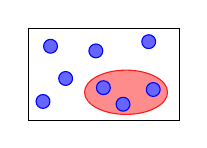
\begin{tikzpicture}
		\begin{axis}[hide axis, xmin=0, xmax=1, ymin=0, ymax=1, clip=false, width=3.5cm,height=2.75cm,]
			\fill[draw=\ldraw, fill opacity=0.5, red!90!white] (0.65,0.30) ellipse (15pt and 8pt);
			\draw[blue, fill=blue!60!white] (0.10, 0.20) circle (2.5pt) (0.15, 0.80) circle (2.5pt) (0.45, 0.75) circle (2.5pt)
																(0.50, 0.35) circle (2.5pt) (0.83, 0.33) circle (2.5pt) (0.80, 0.85) circle (2.5pt)
																(0.25, 0.45) circle (2.5pt) (0.63, 0.17) circle (2.5pt);
			\draw[line width=0.05mm] (axis cs:0,0) rectangle (axis cs:1,1);
		\end{axis}
	\end{tikzpicture}
\end{minipage}%
\begin{minipage}{0.70\linewidth}
	The conditional probability law on $B$, given that $B$ ocurred, is also discrete uniform. Each event inside $B$ would have a probability of $\frac{1}{|B|}$.
	\vspace{1mm} \\
	The conditional probability law on $\Omega$, given that $B$ ocurred, is not discrete uniform. Events outside $B$ have $0$ probability, different from events inside.
\end{minipage}%
}

\sectionbox{\subsubsection{Multiplication Rule}\topline
\vspace{-1mm}
\begin{align*}
	\shortintertext{Notice that:}
		P(A \cap B) &= P(B) P(A|B) \\
					&= P(A) P(B|A) \\
	\shortintertext{And for 3 events we have:}
		P[(A \cap B) \cap C] &= P(A \cap B) P(C|A \cap B) \\
						   &= P(A) P(B|A) P(C|A \cap B)\\
	\shortintertext{More generally:}
		\Aboxed{P\left(\bigcap_{i=1}^{n} A_{i}\right) &= P(A_{1})\prod_{i=2}^{n}P\left(A_{i} \Bigg| \bigcap_{j=1}^{i-1} A_{j} \right)}
\end{align*}\\
A particular intersection of events would be represented as a full path in a probability tree.
}

\sectionbox{\subsubsection{Total Probability Rule}\topline
\begin{itemize}
	\item Consider a partition of $\Omega$ into $A_{i}$ events. Since it's a partition, events are disjoint.
	\item Let's say we have a probability model for $A_{i}$.
	\item We have also modeled $P(B)$ for each scenario, i.e. $P(B|A_{i})$
	\item We can use \textbf{finite additivity} in order to calculate $P(B)$
\end{itemize}
\vspace{-1.5mm}
\begin{minipage}{0.34\linewidth}
	\centering
	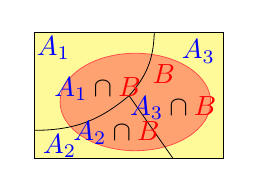
\begin{tikzpicture}[scale=0.8]
		\begin{scope}[line width=0.1mm]
			\fill [yellow!40!white, draw=black] (0, 0) rectangle (3, 2);
			\fill[draw=\ldraw, fill opacity=0.5, red!70!white] (1.6,0.9) ellipse (34pt and 22pt);
			\draw (0, 0.45) to [bend right=20] (1.5, 1);
			\draw (1.5, 1) to [bend right=20] (1.9, 2);
			\draw (1.5, 1) -- (2.2, 0);
			\node at (1, 1.1) {$\Blue{A_{1}} \cap \Red{B}$};
			\node at (2.05, 1.35) {$\Red{B}$};
			\node at (1.3, 0.4) {$\Blue{A_{2}} \cap \Red{B}$};
			\node at (2.2, 0.8) {$\Blue{A_{3}} \cap \Red{B}$};
			\node at (0.3, 1.75) {$\Blue{A_1}$};
			\node at (0.4, 0.2) {$\Blue{A_2}$};
			\node at (2.6, 1.70) {$\Blue{A_3}$};
		\end{scope}
	\end{tikzpicture}
\end{minipage}%
\begin{minipage}{0.66\linewidth}
	\begin{flalign*}
		P(B) &= P(B \cap A_{1}) + P(B \cap A_{2}) + P(B \cap A_{3}) &\\
			 &= P(A_1)P(B|A_1) + ... + P(A_3)P(B|A_3)
	\end{flalign*}

	By induction, for a \textit{2-level probability scenario}, it can be proven that: \vspace{0.75mm}

	{\centering \boxed{P(B) = \sum_{i=1}P(A_i)P(B|A_i)}\\}
\end{minipage}%
}

\sectionbox{\subsubsection{Multiplication \& Total Probability Rules: Tree Interpretation}\topline
Consider the following 3-level probability tree (scenario): $A_1, A_2$ are disjoint, $B_1, B_2$ are disjoint, $C_1, C_2$ are disjoint,
then $B_1$'s total probability is calculated using both rules: \\\vspace{1mm}
\centering
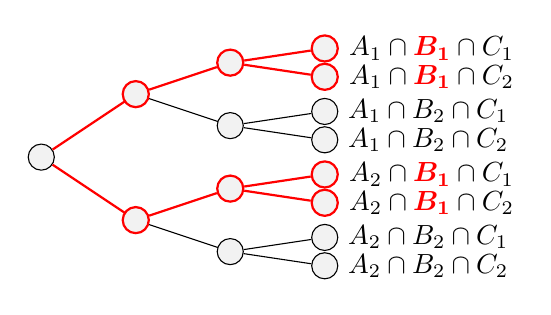
\begin{tikzpicture}[scale=0.40, grow=right,
				level 1/.style={sibling distance=-4cm, level distance=3cm},
				level 2/.style={sibling distance=-2cm},
				level 3/.style={sibling distance=-0.9cm},
				probability/.style={above, midway},
				event/.style={circle, draw, fill=gray!10, minimum size=0.08cm}]
	\node[event] {}
	child { [draw=red, thick] node[event] {} 
		child { node[event] {} 
			child { node[event, label=right:{$A_1 \cap \boldsymbol{\Red{B_1}} \cap C_1$}] {} edge from parent node[above, pos=0.5] {} }
			child { node[event, label=right:{$A_1 \cap \boldsymbol{\Red{B_1}} \cap C_2$}] {} edge from parent node[above, pos=0.5] {} }
			edge from parent node[above, pos=0.5] {}
		}
		child { [draw=black, thin] node[event] {}
			child {node[event, label=right:{$A_1 \cap B_2 \cap C_1$}] {} edge from parent node[above, pos=0.5] {} }
			child {node[event, label=right:{$A_1 \cap B_2 \cap C_2$}] {} edge from parent node[above, pos=0.5] {} }
			edge from parent node[below, pos=0.5] {}
		}
		edge from parent node[] {}
	}
	child { [draw=red, thick] node[event] {}
		child {  node[event] {}
			child { node[event, label=right:{$A_2 \cap \boldsymbol{\Red{B_1}} \cap C_1$}] {} edge from parent node[above, pos=0.5] {} }
			child { node[event, label=right:{$A_2 \cap \boldsymbol{\Red{B_1}} \cap C_2$}] {} edge from parent node[above, pos=0.5] {} }
			edge from parent node[above, pos=0.5] {}
		}
		child { [draw=black, thin] node[event] {}
			child {node[event, label=right:{$A_2 \cap B_2 \cap C_1$}] {} edge from parent node[above, pos=0.5] {} }
			child {node[event, label=right:{$A_2 \cap B_2 \cap C_2$}] {} edge from parent node[above, pos=0.5] {} }
			edge from parent node[above, pos=0.5] {}
		}
		edge from parent
		node[] {}
	};
\end{tikzpicture}
}

\examplebox{
Consider the following events: $A:$ Airplane is flying above, $B:$ Something registers on the radar screen. Some conditional probabilities are depicted in the figure,
e.g. $P(B|A)=0.99$. Find the probability that there's an airplane flying above, given that the radar registers something.
\begin{minipage}{0.60\linewidth}
	\centering
	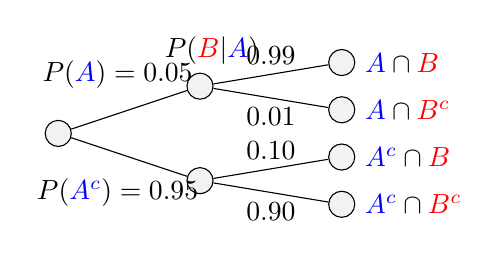
\begin{tikzpicture}[scale=0.60, grow=right, level 1/.style={sibling distance=-2cm, level distance=3cm}, level 2/.style={sibling distance=-1cm},
    				probability/.style={above, midway},
					event/.style={circle, draw, fill=gray!10, minimum size=0.08cm}]
		\node[event] {}
		child {node[event] {} 
			child {node[event, label=right:{$\Blue{A} \cap \Red{B}$}] {} 
				edge from parent
				node[above, pos=0.5] {$0.99$}
			}
			child {node[event, label=right:{$\Blue{A} \cap \Red{B^c}$}] {} 
				edge from parent 
				node[below, pos=0.5] {$0.01$}
			}
			edge from parent
			node[above, midway, pos=0.40, yshift=2mm] {$P(\Blue{A})=0.05$}
		}
		child {node[event] {}
			child {node[event, label=right:{$\Blue{A^c} \cap \Red{B}$}] {}
				edge from parent
				node[above, pos=0.5] {$0.10$}
			}
			child {node[event, label=right:{$\Blue{A^c} \cap \Red{B^c}$}] {}
				edge from parent
				node[below, pos=0.5] {$0.90$}
			}
			edge from parent
			node[below, midway, pos=0.40, yshift=-2mm] {$P(\Blue{A^{c}})=0.95$}
		};
		\node [] at (3.25, 1.75) {$P(\textcolor{red}{B}|\textcolor{blue}{A})$};
	\end{tikzpicture}
\end{minipage}%
\begin{minipage}{0.40\linewidth}
	\begin{flalign*}
		P(A\cap B) & = P(A)\,P(B|A) & \\
				   & = (0.05)(0.99) \\
				   \\
		P(B) & = (0.05)(0.99)\, + & \\
				   & \quad\quad (0.95)(0.10) \\
				   & = 0.1445 \\
					\\
		P(A | B)   & = \frac{(0.5)(0.99)}{0.1445} & \\
				   & = 0.34
	\end{flalign*}
\end{minipage}%
}

\sectionbox{\subsubsection{Bayes' Rule}\topline
\begin{itemize}
	\item Consider a partition of $\Omega$ into $A_{i}$ disjoint events.
	\item We have an initial model or beliefs for $A_{i}$.
	\item We know how likely it is a particular event $B$ under each scenario, i.e. $P(B|A_{i})$.\\ \vspace{0.5mm}
			$\Blue{A_{i}} \xrightarrow[P(\Red{B}|\Blue{A_{i}})]{\text{model}} \Red{B}$ \vspace{0.5mm}
	\item Given that $B$ occurred, we can update our model: Analyze possible causes or most likely scenarios for $B$. \\ \vspace{0.5mm}
			$\Red{B} \xrightarrow[P(\Blue{A_{i}}|\Red{B})]{\text{inference}} \Blue{A_i}$ \vspace{0.5mm}
	\item In other words, we use inference to analyze how likely is a scenario $A_{i}$, given that $B$ occurred.
\end{itemize}
\vspace{0.5mm}
\begin{minipage}{0.34\linewidth}
	\centering
	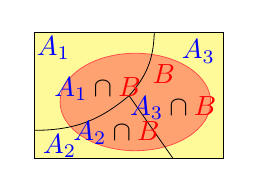
\begin{tikzpicture}[scale=0.8]
		\begin{scope}[line width=0.1mm]
			\fill [yellow!40!white, draw=black] (0, 0) rectangle (3, 2);
			\fill[draw=\ldraw, fill opacity=0.5, red!70!white] (1.6,0.9) ellipse (34pt and 22pt);
			\draw (0, 0.45) to [bend right=20] (1.5, 1);
			\draw (1.5, 1) to [bend right=20] (1.9, 2);
			\draw (1.5, 1) -- (2.2, 0);
			\node at (1, 1.1) {$\Blue{A_{1}} \cap \Red{B}$};
			\node at (2.05, 1.35) {$\Red{B}$};
			\node at (1.3, 0.4) {$\Blue{A_{2}} \cap \Red{B}$};
			\node at (2.2, 0.8) {$\Blue{A_{3}} \cap \Red{B}$};
			\node at (0.3, 1.75) {$\Blue{A_1}$};
			\node at (0.4, 0.2) {$\Blue{A_2}$};
			\node at (2.6, 1.70) {$\Blue{A_3}$};
		\end{scope}
	\end{tikzpicture}
\end{minipage}%
\begin{minipage}{0.66\linewidth}
	\begin{align*}
		P(A_{i}|B) &= \frac{P(A_{i} \cap B)}{P(B)} \\
			 \Aboxed{P(A_{i}|B) &= \frac{P(A)P(B|A_{i})}{\sum_{j}P(A_j)P(B|A_j)}} 
	\end{align*}
\end{minipage}\vspace{1.5mm}\\
Check the diagrams: \url{https://en.wikipedia.org/wiki/Bayes%27_theorem#Random_variables}
}

\subsection{Independence}
\sectionbox{\subsubsection{When Conditional Probability = Unconditional Probability}\topline
Consider 3 tosses of a biased coin: $P(H)=p, P(T)=1-p$ \\ \vspace{1mm}
\begin{minipage}{0.50\linewidth}
	\centering
	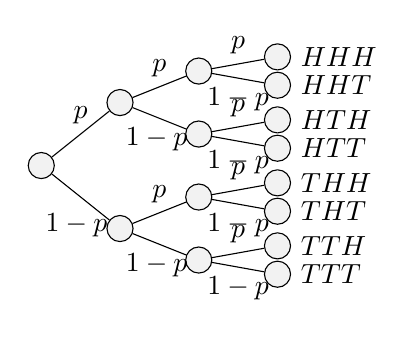
\begin{tikzpicture}[scale=0.40, grow=right,
					level 1/.style={sibling distance=-4cm, level distance=2.5cm},
					level 2/.style={sibling distance=-2cm},
					level 3/.style={sibling distance=-0.9cm},
					probability/.style={above, midway},
					event/.style={circle, draw, fill=gray!10, minimum size=0.08cm}]
		\node[event] {}
		child { node[event] {} 
			child { node[event] {} 
				child { node[event, label=right:{$HHH$}] {} edge from parent node[above, pos=0.5] {$p$} }
				child { node[event, label=right:{$HHT$}] {} edge from parent node[below, pos=0.5] {$1-p$} }
				edge from parent node[above, pos=0.5] {$p$}
			}
			child { node[event] {}
				child {node[event, label=right:{$HTH$}] {} edge from parent node[above, pos=0.5] {$p$} }
				child {node[event, label=right:{$HTT$}] {} edge from parent node[below, pos=0.5] {$1-p$} }
				edge from parent node[below, pos=0.5, xshift=-1pt] {$1-p$}
			}
			edge from parent node[above, pos=0.5] {$p$}
		}
		child { node[event] {}
			child {  node[event] {}
				child { node[event, label=right:{$THH$}] {} edge from parent node[above, pos=0.5] {$p$} }
				child { node[event, label=right:{$THT$}] {} edge from parent node[below, pos=0.5] {$1-p$} }
				edge from parent node[above, pos=0.5] {$p$}
			}
			child { node[event] {}
				child {node[event, label=right:{$TTH$}] {} edge from parent node[above, pos=0.5] {$p$} }
				child {node[event, label=right:{$TTT$}] {} edge from parent node[below, pos=0.5] {$1-p$} }
				edge from parent node[below, pos=0.5, xshift=-1pt] {$1-p$}
			}
			edge from parent
			node[below, pos=0.5, yshift=-2.5pt, xshift=-1.5pt] {$1-p$}
		};
	\end{tikzpicture}
\end{minipage}%
\begin{minipage}{0.50\linewidth}
	Notice that the unconditional and conditional probabilities for $H_2$ (heads in the second toss) are the same:
	\begin{align*}
		\shortintertext{Conditional Probability (from the diagram)}
			P(H_{2}|H_{1}) = & \; P(H_{2}|T_{1}) = p \\
		\shortintertext{Unconditional Probability (using Total Probability)}
			P(H_2) = & \; P(H_1)P(H_2|H_1) + \\
					 & \; P(T_1)P(H_2 | T_1) \\
				   = & \; (p)(p) + (1-p)(p) \\
				   = & \; p
	\end{align*} 
\end{minipage}%
}

\sectionbox{\subsubsection{Independence of Two Events}\topline
Intuitive definition: $P(B|A)=P(B) \then$ The ocurrence of $A$ gives no new information about $B$.\\
\vspace{1.5mm}
Formal definition:\\
{\centering\fbox{%
\begin{minipage}{0.4\linewidth}
Two events are independent if:\\ \vspace{-0.5mm}
\begin{equation*}
    P(A \cap B) = P(A)P(B)
\end{equation*}
\end{minipage}}\\}%
\vspace{1.5mm}
This definition symmetrically implies both $P(B|A)=P(B)$ and $P(A|B)=P(A)$ and works even when $P(A)=0$.\\
}

\sectionbox{\subsubsection{Why $P(A \cap B)=P(A)P(B) \iff$ Independence}\topline
So far we know the following: \vspace{-1mm}
\begin{align*}
	\text{Independent}(A,B) &\then P(A\cap B)=P(A|B)P(B)=P(A)P(B) \\
	\text{Dependent}(A,B) &\then P(A\cap B)=P(A|B)P(B) \neq P(A)P(B)
\end{align*} \vspace{-1mm}
If by pure coincidence we have \vspace{-1mm}
\begin{align*}
	\text{Dependent}(A,B) \AND P(A\cap B)=P(A)P(B)
\end{align*} \vspace{-1mm}
Then that would imply both: \vspace{-1mm}
\begin{align*}
	P(A|B)P(B)&=P(A)P(B) \\
	P(A|B)P(B)&\neq P(A)P(B) \quad \text{(a contradiction)}
\end{align*} \vspace{-3.5mm}
}

\sectionbox{\subsubsection{Independence of "Essentially Deterministic" Events}\topline
{\centering\fbox{%
\begin{minipage}{0.9\linewidth}
$P(A)=0 \OR P(A)=1 \then A$ is independent of any event and independent of itself.
\end{minipage}}\\}%
\vspace{1mm}
Let $B$ be any event $\then P(A \cap B)=P(A)P(B)$ for both cases $P(A)=0 \AND P(A)=1 \qed $
}

\sectionbox{\subsubsection{Independence and Disjoint Sets}\topline
\begin{itemize}
	\item Let $A$ and $B$ be disjoint events $\then P(A \cap B)=0$.
	\item Let $P(A), P(B) > 0 \then P(A)P(B)>0$
	\item Therefore $P(A \cap B)=P(A)P(B)$ does not hold $\then$ Events are not independent.
\end{itemize}
\vspace{1.5mm}
\begin{minipage}{0.25\linewidth}
	\centering
	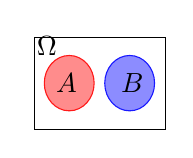
\begin{tikzpicture}
		\begin{axis}[hide axis, xmin=0, xmax=1, ymin=0, ymax=1, clip=false, width=3.25cm,height=2.75cm,]
			\fill[draw=\ldraw, fill opacity=0.5, red!90!white] (0.27, 0.5) ellipse (9pt and 10pt);
			\fill[draw=\ldraw, fill opacity=0.5, blue!90!white] (0.73, 0.5) ellipse (9pt and 10pt);
			\node at (0.25, 0.5) {$A$};
			\node at (0.75, 0.5) {$B$};
			\node at (0.1, 0.9) {$\Omega$};
			\draw[line width=0.05mm] (axis cs:0,0) rectangle (axis cs:1,1);
		\end{axis}
	\end{tikzpicture}
\end{minipage}%
\begin{minipage}{0.73\linewidth}
	Being independent is something completely different from being disjoint. Furthermore, for mutually exclusive, disjoint events with positive probabilities, 
	if $A$ occurs $\then$ $B$ can't occur, so it gives us a lot of information. Therefore:
	\bcentering{\textbf{Disjoint events are not independent}} \vspace{-2mm}
	\bcentering{\textbf{Independence is a relation about information}}
	If one of the events is impossible $\then$ They are \textbf{trivially independent}.
\end{minipage}
}

\examplebox{
We have a peculiar coin. When tossed twice, the first toss results in $H$ with probability $1/2$. However, the second toss always yields the same result as the first toss.
Thus, the only possible outcomes for a sequence of $2$ tosses are $HH$ and $TT$, and both have equal probabilities. Are the two events $A={H_1}$ and $B={H_2}$ independent?\\
\vspace{1.5mm}
$P(A)=P(B)=P(A \cap B) = 1/2 \then P(A \cap B) \neq P(A)P(B) \then$ Not independent.
}

\examplebox{
Let $A \subset \Omega \then P(A \cap \Omega) = P(A) \then P(A \cap \Omega)=P(A)P(\Omega) \then$ Independent.\\
\vspace{1.5mm}
Let $0<P(A)<1 \then P(A \cap A) = P(A) \neq P(A)P(A) \then$ Not independent.
}

\sectionbox{\subsubsection{Independence of Complements}\topline
Let $A$ and $B$ be independent, then:\\
\vspace{-2mm}
\begin{minipage}{0.23\linewidth}
	\centering
	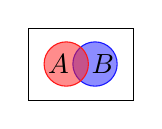
\begin{tikzpicture}
		\begin{axis}[hide axis, xmin=0, xmax=1, ymin=0, ymax=1, clip=false, width=2.8cm,height=2.5cm,]
			\fill[draw=\ldraw, fill opacity=0.5, blue!90!white] (0.7, 0.5) circle (8pt);
			\fill[draw=\ldraw, fill opacity=0.5, red!90!white] (0.4, 0.5) circle (8pt);
			\draw[line width=0.05mm] (axis cs:0,0) rectangle (axis cs:1.1,1);
			\node at (0.32, 0.5) {$A$};
			\node at (0.78, 0.5) {$B$};
		\end{axis}
	\end{tikzpicture}
\end{minipage}%
\begin{minipage}{0.78\linewidth}
	\begin{flalign*}
			A &=  \textcolor{purple}{(A \cap B)} \cup \textcolor{red!90}{(A \cap B^c)}  && \\
			P(A) &=  P(A \cap B) + P(A \cap B^c) \quad\quad \text{(since they're disjoint)} \\
			P(A) &= P(A)P(B) + P(A \cap B^c) \\
			P(A \cap B^c) &= P(A) - P(A)P(B) = P(A)(1 - P(B))
	\end{flalign*}
\end{minipage}%
\bcentering{P\left(A \cap B^c\right) = P\big(A\big)P\left(B^c\right)}
By the same logic: $A$ and $B$ independent $\then$ $A$ and $B^c$ independent $\then$ $B^c$ and $A$ independent $\then$ $B^c$ and $A^c$ independent $\then$ $A^c$ and $B^c$ independent.
\bcentering{P\left(A^c \cap B^c\right) = P\left(A^c\right)P\left(B^c\right)}
}

\sectionbox{\subsubsection{Conditional Independence}\topline
{\centering\fbox{%
\begin{minipage}{0.7\linewidth}
Given an event $C$, events $A$ and $B$ are conditionally independent if:\\ \vspace{-0.5mm}
\begin{equation*}
    P(A \cap B | C) = P(A|C)P(B|C)
\end{equation*}
\end{minipage}}\\}%
\vspace{1.5mm}
Now, notice that by the Bayes' Rule and Multiplication Rule: \\\vspace{1mm}
$P(A\cap B|C) = \frac{P(A \cap B \cap C)}{P(B)}  = \frac{P(C)P(B|C)P(A|B \cap C)}{P(C)}= P(B|C)P(A|B\cap C)$ \\\vspace{1mm}
So conditional independence also implies: \, \boxed{P(A|B \cap C) = P(A|C)} \\ \vspace{1mm}
In words, this relation states that if $C$ is known to have occurred, the additional knowledge that $B$ also occurred does not change the probability of $A$.
}

\sectionbox{\subsubsection{Independence does not imply Conditional Independence}\topline
\begin{minipage}{0.25\linewidth}
	\centering
	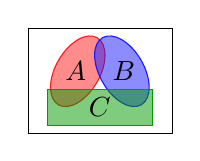
\begin{tikzpicture}
		\begin{axis}[hide axis, xmin=0, xmax=1, ymin=0, ymax=1, clip=false, width=2.8cm,height=2.5cm,]
			\fill[draw=\ldraw, rotate around={150:(0.27, 0.5)}, fill opacity=0.5, red!90!white] (0.27, 0.5) ellipse (8pt and 14pt);
			\fill[draw=\ldraw, rotate around={30:(0.73, 0.5)}, fill opacity=0.5, blue!90!white] (0.73, 0.5) ellipse (8pt and 14pt);
			\fill[draw=\ldraw, fill opacity=0.5, green!60!black] (-0.05,-0.25) rectangle (1.05,0.25);
			\draw[line width=0.05mm] (axis cs:-0.25,-0.35) rectangle (axis cs:1.25,1.1);
			\node at (0.25, 0.5) {$A$};
			\node at (0.75, 0.5) {$B$};
			\node at (0.5, 0) {$C$};
		\end{axis}
	\end{tikzpicture}
\end{minipage}%
\begin{minipage}{0.74\linewidth}
	For any probabilistic model, let $A$ and $B$ be independent events, and let $C$ be an event such that $P(C) > 0, P(A | C) > 0$, and $P(B | C) > 0$,
	while $A \cap B \cap C = \emptyset$ \vspace{1.5mm}\\ 
	$\then A$ and $B$ can't be conditionally independent since $ P(A \cap B | C) = 0$ while $P(A | C)P(B | C) > O \qed$.
\end{minipage}
}

\examplebox{
Consider two independent fair coin tosses, in which all four possible outcomes are equally likely.\\
Let $H_1$ = \{ 1st toss is a head\}, $H_2$ = \{2nd toss is a head\}, $D$ = \{the two tosses have different results\}. Then events $H_1$ and $H_2$ are (unconditionally) independent, 
and $P(H_1|D)=P(H_2|D)=1/2$, but since $P(H_1 \cap H_2 | D) = 0 \then P(H_1 \cap H_2 | D) \neq P(H_1|D)P(H_2|D)$.
}

\sectionbox{\subsubsection{Conditional Independence does not imply Independence}\topline
\begin{minipage}{0.25\linewidth}
	\centering
	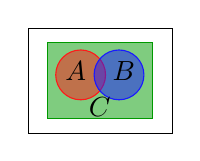
\begin{tikzpicture}
		\begin{axis}[hide axis, xmin=0, xmax=1, ymin=0, ymax=1, clip=false, width=2.8cm,height=2.5cm,]
			\fill[draw=\ldraw, fill opacity=0.5, green!60!black] (-0.05, -0.15) rectangle (1.05,0.90);
			\fill[draw=\ldraw, fill opacity=0.5, red!90!white] (0.3, 0.45) circle (9pt);
			\fill[draw=\ldraw, fill opacity=0.5, blue!90!white] (0.7, 0.45) circle (9pt);
			\draw[line width=0.05mm] (axis cs:-0.25,-0.35) rectangle (axis cs:1.25,1.1);
			\node at (0.25, 0.5) {$A$};
			\node at (0.75, 0.5) {$B$};
			\node at (0.5, 0) {$C$};
		\end{axis}
	\end{tikzpicture}
\end{minipage}%
\begin{minipage}{0.74\linewidth}
	Let $A,B$ be conditionally independent given $C$:\\
	$P(A\cap B|C)=P(A|C)P(B|C)$ \\
	$\then P(A\cap B|C^c)=P(A|C^c)P(B|C^c)$.\\
	By total probability we have:\\
	$P(A)=P(C)P(A|C) + P(C^c)P(A|C^c)$ and \\
	$P(B)=P(C)P(B|C) + P(C^c)P(B|C^c)$.
\end{minipage} \vspace{1mm}\\
The unconditional probability of $A \cap B = P(C)P(A\cap B|C) + P(C^c)P(A\cap B|C^c)$, \; so
$P(A \cap B) = P(C)P(A|C)P(B|C) + P(C^c)P(A|C^c)P(B|C^c)$, \; therefore
$P(A \cap B) = P(A)P(B)$ is not necessarily true $\qed$
}

\examplebox{
Let $A$ and $B$ be conditionally independent given $C \then P(A \cap B | C) = P(A | C)P(B | C)$. \\
Let $P(C) = 1/2$ and $P(A|C)=P(B|C)=1/2$, and also $P(A|C^c)=P(B|C^c)=0$. So $P(A \cap B) = P(C)P(A\cap B|C) + P(C^c)P(A \cap B |C^c) = (1/2)^3 + 0 = 1/8$. \\\vspace{1mm}
But $P(A)P(B) = \Red{[}P(C)P(A|C) + P(C^c)P(A|C^c)\Red{]}\Red{[}P(C)P(B|C) + P(C^c)P(B|C^c)\Red{]}$ $= (1/2)(1/2)= 1/4 \then P(A \cap B) \neq P(A)P(B)$
}

\sectionbox{\subsubsection{Conditional Independence \& Complements}\topline
Let $A$ and $B$ be \textbf{independent and conditionally independent} given $C$. Let $P(C), P(C^c) > 0$ \\
$\then A$ and $B^c$ are guaranteed to be conditionally independent given $C$. Proof:\\ \vspace{1mm}

We need to get to the target equation: $P(A \cap B^c | C) = P(A|C)P(B^c|C)$. Notice that:\\
$P(B) + P(B^c) = 1 \then P(B|C) + P(B^c|C) = 1 \then P(B^c|C)=1-P(B|C)$. \\
Now, $(A\cap B)$ and $(A \cap B^c)$ are disjoint events (they can't both occur) $\then (A\cap B) \cup (A \cap B^c) = A$ 
(this can be proven using the properties of sets, but try to see it intuitively). Therefore $P(A \cap B^c|C) = P(A|C) - P(A\cap B|C)$.\\ \vspace{1mm}

Considering the assumptions, the target equation can now be expressed as:\\
$P(A|C) - P(A\cap B|C) = P(A|C)[1 - P(B|C)]$\\
$P(A|C) - P(A|B)P(B|C) = P(A|C) - P(A|C)P(B|C) \qed$

\vspace{1mm}
\topline
$A$ and $B$ are not guaranteed to be conditionally independent given $C^c$. This may be true in some special cases, e.g., if $P(A)=0$ and $P(B)=0$. 
However, it is in general false. Suppose, for example, that events $A$ and $B$ have nonempty intersection inside $C$, 
and are conditionally independent, but have empty intersection inside $C^c$ , which would make them dependent (given $C^c$).
}

\examplebox{\subsubsection{Conditioning may affect Independence}\topline
Consider two unfair coins $A$ and $B$ with $P(H|A)=0.9, P(H|B)=0.1$. Given a particular coin, tosses are independent. Also, coins are equally likely to be chosen.
Are overall coin tosses independent? \\\vspace{1mm}

Consider the particular result ${H_{11}}$. Let $H^{10}={H_{1}\cap...\cap H_{10}}$\\
Unconditional probability:\\
$P(H_{11})=P(A)P(H_{11}|A) + P(B)P(H_{11}|B)=(0.5)(0.9)+(0.5)(0.1)=\Blue{0.5}$\\
Conditional probability (given that the first 10 results are H):\\
$P(H_{11}|H^{10}) = \frac{P(H_{11}\cap H^{10})}{P(H^{10})}$\\
$P(H_{11}|H^{10}) = \frac{P(A)P(H^{10}\cap H_{11}|A) + P(B)P(H^{10} \cap H_{11}|B)}{P(A)P(H^{10}|A) + P(B)P(H^{10}|B)}$\\
$P(H_{11}|H^{10}) = \frac{(0.9^{11})(0.5)+(0.1^{11})(0.5)}{(0.9^{10})(0.5)+(0.1^{10})(0.5)} \approx \Blue{0.9} \then$ \Blue{Overall tosses aren't independent.}
}

\sectionbox{\subsubsection{Collective/Mutual Independence}\topline
{\centering\fbox{%
\begin{minipage}{0.95\linewidth}
Events $A_1, A_2,..., A_n$ are called independent if:\\ \vspace{-0.5mm}
\begin{equation*}
    P\left(\bigcap_{i\in S}A_i \right) = \prod_{i \in S} P(A_i), \quad \text{for every subset } S \; \text{of } \{1,2,...,n\}
\end{equation*}
\end{minipage}}\\}%
\vspace{1.5mm}
For instance, let $n=3$, then we'll need the following Pairwise Independence conditions:\\ \vspace{1mm}
$P(A_1 \cap A_2)=P(A_1)P(A_2)$\\
$P(A_1 \cap A_3)=P(A_1)P(A_3)$\\
$P(A_2 \cap A_3)=P(A_2)P(A_3)$\\\vspace{1mm}
But we'll also need: $P(A_1 \cap A_2 \cap A_3)=P(A_1)P(A_2)P(A_3)$, since it doesn't follow from the Pairwise Independence condition. \\\vspace{1.5mm}
Furthermore, if the boxed condition holds, then any relation such as: $P(A_{3})=P(A_{3}|A_{1} \cap A_{2}) = P(A_{3}|A_{1} \cap A_{2}^{c}) = P(A_{3}|A_{1}^{c} \cap A_{2})...$
also holds.\\\vspace{1.5mm}
\Red{For a \textbf{very detailed and long} sequence of proofs see:}
\url{https://stats.libretexts.org/Bookshelves/Probability_Theory/Probability_Mathematical_Statistics_and_Stochastic_Processes_(Siegrist)/02%3A_Probability_Spaces/2.05%3A_Independence}\\
\Red{and}\\
\url{https://math.stackexchange.com/questions/1889772/understanding-the-definition-for-collections-of-events-being-independent}\\
\Red{Add the proofs to the appendix!}
}


\examplebox{
Let $A, B, C, D$ be independent events.\\
a) Is it guaranteed that $A \cap C$ is independent from $B^{c} \cap D$?\\
$A \cap C$ only gives information about $A$ and $C$, and nothing about $D$ or $B$ (and therefore $B^c$).\\\vspace{1mm}
b) Is it guaranteed that $A \cap B^c \cap D$ is independent from $B^{c} \cap D^c$?\\
If $A \cap B^c \cap D$ occurs $\then D$ occurs $\then D^c$ doesn't occur, and so it affects the probability of $B^{c} \cap D^c$.
Also, consider that if $B^c \cap D \neq \emptyset \then$ It's a subset of $B^{c} \cup D^c$ and they have common elements, 
but we're not considering the intersection with $A$ that could exclude it.
}

\examplebox{\subsubsection{Pairwise Independent, but not Collectively Independent}\topline
Consider two independent fair coin tosses $\then$ Outcomes in \{HH, HT, TH, TT\} have the same probability.\\
Let \{$H_{1}=$ First toss is $H$\}, \{$H_{2}=$ Seconds toss is $H\} \then P(H_1)=P(H_2)=1/2$\\
Let $C:$ The two tosses have the same result.\\\vspace{1.5mm}

There's pairwise independence between all pairs:\\
$P(H_1 \cap C)=P(H_1 \cap H_2)=1/4 \AND P(H_{1})P(C)=(1/2)(1/2)=1/4$\\
$P(H_2 \cap C)=P(H_2 \cap H_1)=1/4 \AND P(H_{2})P(C)=(1/2)(1/2)=1/4$\\\vspace{1.5mm}

But there's no independence for the conjunction of all three events:\\
$P(H_1 \cap H_2 \cap C) = P(H_1 \cap H_2) = (1/2)^{2}=1/4$\\
$P(H_1)P(H_2)P(C)=(1/2)^{3}=1/8$\\\vspace{1.5mm}

Intuitively, notice that for $P(C|H_1)$, the occurrence of $H_1$ doesn't give any new information, since the second toss could still be $T$ or $H$ with equal probability, 
so $P(C|H_1)=(1/2)=P(C)$, but if we are asked for $P(C|H_1 \cap H_2)$ we can see that the answer is $1$.
}

\sectionbox{\subsubsection{Reliability: Serial Configuration}\topline
Let $U_i$ be the event in which the \textit{ith} unit is up with probability $p_i$.\\
\vspace{1.5mm}
{\centering
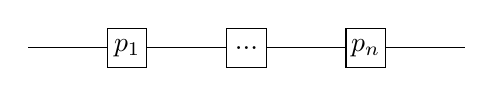
\begin{tikzpicture}[square/.style={draw, thin, black, minimum size=5mm}]
	\node[square, label=center:$p_1$] (s1) at (0,0) {};
	\node[square, label=center:$...$, right=of s1] (s2) {};
	\node[square, label=center:$p_n$, right=of s2] (s3) {};
	\draw[thin, -] ($(s1.west) - (1,0)$) -- (s1.west); % [thin, -] ----> "-" means there will be no arrowhead
	\draw[thin, -] (s1) -- node[above] {} (s2);
	\draw[thin, -] (s2) -- node[above] {} (s3);
	\draw[thin, -] (s3.east) -- ($(s3.east) + (1,0)$);
\end{tikzpicture}\\}
\vspace{1mm}
Events $U_i$ are independent, so the probability that the whole serial system is up becomes: 
\bcentering{P\left(\bigcap U_i\right)=\prod p_i}
}

\sectionbox{\subsubsection{Reliability: Parallel Configuration}\topline
Notice that the system is up if any subset (of the set of all components) is up. Let $F_{i}$ be the event in which the \textit{ith} component fails (these events are also independent), then:
\\\vspace{1.5mm}
\begin{minipage}{0.4\linewidth}
	\centering
	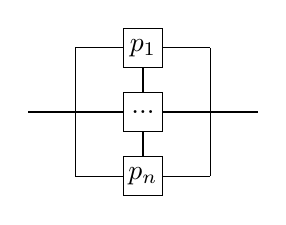
\begin{tikzpicture}[square/.style={draw, thin, black, minimum size=5mm}]
		\node[square, label=center:$p_1$] (s1) at (0,0) {};
		\node[square, label=center:$...$, below=3mm of s1] (s2) {};
		\node[square, label=center:$p_n$, below=3mm of s2] (s3) {};
		\draw[thin, -] ($(s1.west) - (0.60,0)$) -- (s1.west); % [thin, -] ----> "-" means there will be no arrowhead
		\draw[thin, -] ($(s1.west) - (0.60,0)$) -- ($(s2.west) - (0.60,0)$);
		\draw[thin, -] ($(s2.west) - (1.2,0)$) -- (s2.west);
		\draw[thin, -] ($(s2.west) - (0.60,0)$) -- ($(s3.west) - (0.60,0)$);
		\draw[thin, -] ($(s3.west) - (0.60,0)$) -- (s3.west);
		\draw[thin, -] (s1) -- node[above] {} (s2);
		\draw[thin, -] (s2) -- node[above] {} (s3);
		\draw[thin, -] (s1.east) -- ($(s1.east) + (0.60,0)$);
		\draw[thin, -] ($(s1.east) + (0.60,0)$) -- ($(s2.east) + (0.60,0)$);
		\draw[thin, -] (s2.east) -- ($(s2.east) + (1.2,0)$);
		\draw[thin, -] ($(s2.east) + (0.60,0)$) -- ($(s3.east) + (0.60,0)$);
		\draw[thin, -] (s3.east) -- ($(s3.east) + (0.60,0)$);
	\end{tikzpicture}
\end{minipage}
\begin{minipage}{0.55\linewidth}
	The probability that the whole system is up becomes $P\left(\bigcup U_i\right)$, which can be seen as the complementary probability that all components fail together:
	\vspace{0.5mm}\\
	$1 - P\left(\bigcap F_i\right) = 1 - \prod P(F_i)$
	\bcentering{1-\prod(1-p_i) }
\end{minipage}
}

\examplebox{\subsubsection{Reliability: Complex Configuration}\topline
Assume each component has a probability $p$ of \textit{being up}.\\
\vspace{1mm}
{\centering
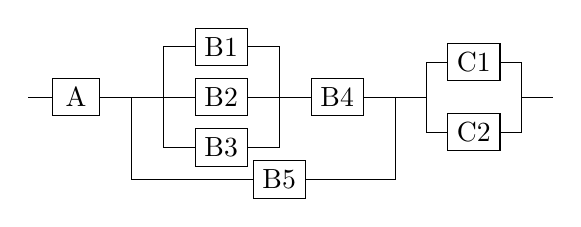
\begin{tikzpicture}[-,auto,node distance=10mm]
	\tikzstyle{point}=[coordinate]
	\tikzstyle{block}=[draw, rectangle, minimum height=3mm, minimum width=6mm]
	% Points and Blocks
	\node[point] (p0)                     		{};
	\node[block] (A)	[right = 3mm of p0]		{A};
	\node[point] (p1)	[right = 4mm of A]		{};
	\node[point] (p2)   [right = 4mm of p1]		{};
	\node[block] (B2)	[right = 4mm of p2]		{B2};
	\node[block] (B1)	[above = 1.5mm of B2]	{B1};
	\node[block] (B3)	[below = 1.5mm of B2]	{B3};
	\node[point] (p3)   [right = 4mm of B2]		{};
	\node[block] (B4)	[right = 4mm of p3]		{B4};
	\node[block] (B5)	[below = 8mm of p3]		{B5};
	\node[point] (p4)   [right = 4mm of B4]		{};
	\node[point] (p5)   [right = 4mm of p4]		{};
	\node[point] (p6)   [right = 6mm of p5]		{};
	\node[point] (p7)   [right = 6mm of p6]		{};
	\node[point] (p8)   [right = 4mm of p7]		{};
	\node[block] (C1)	[above = 2mm of p6]		{C1};
	\node[block] (C2)	[below = 2mm of p6]		{C2};
	% Straight Lines
	\draw [thin] (p0) -- (A) (A) -- (p1) (p1) -- (p2) (p2) -- (B2) (B2) -- (p3) (p3) -- (B4) (B4) -- (p4) (p4) -- (p5) (p7) -- (p8);
	% Other lines
	\draw [thin] (p2) |- (B1) (p2) |- (B3) (p3) |- (B1) (p3) |- (B3) (p1) |- (B5) (B5) -| (p4) (p5) |- (C1) (p5) |- (C2) (C1) -| (p7) (C2) -| (p7); 
\end{tikzpicture}\\}
\vspace{1.5mm}
The system can be seen as a serial configuration of 3 major groups: $A$, $B$, and $C$. $A$ has probability $p$ of being up, $C$ has probability $1-(1-p)^2$ of being up.
Now, $B$ is a parallel configuration of 2 subgroups: \\
\begin{itemize}
	\item B1, B2, B3 with probability $1-(1-p)^3$ in a serial configuration with B4 (probability $p$),\\
			therefore we have: $\Blue{[1-(1-p)^3]p}$
	\item B5 with probability $\Red{p}$
\end{itemize}
And so, for the group B we have: $1 - (1-\Blue{[1-(1-p)^3p}])(1-\Red{p})$. Finally, this is multiplied by the probabilities of groups A and C.
}

\titlebox{\section{Counting}}

\sectionbox{\subsubsection{Discrete Uniform Probability Law}\topline
If $\Omega$ consists of $n$ equally likely elements $(P({\omega})=1/n)$ and $A$ consists of $k$ elements, then
\bcentering{P(A)=\frac{k}{n}}
}

\sectionbox{\subsubsection{Basic Counting Principles}\topline
If there are $r$ stages and $n_i$ choices at stage $i$, then the number of choices is:
\bcentering{n_{1}n_{2}...n_{r}=\prod_{i=1}^{r} n_i}
}

\examplebox{\subsubsection{Number of subsets of $\{1,...,n\}$}\topline
\vspace{0.5mm}
\begin{minipage}{0.3\linewidth}
	\centering
	\begin{tabular}{|c|c|c|c|c|} 
		\hline
		 1 &  2 & 3 & ... &  n \\
		\hline 
		Y & Y & Y & ... & Y \\ 
		N & N & N & ... & N \\ 
		\hline
	\end{tabular}\\
\end{minipage}
\begin{minipage}{0.65\linewidth}
	Consider the set $\{1,...,n\}$, then all subsets (including $\emptyset$) can be formed by making consecutive binary decisions to include (Y) or not include (N) an element.
	\bcentering{\text{Number of subsets}=2^n}
\end{minipage}
}

\sectionbox{\subsubsection{Permutations}\topline
Number of ways of ordering $n$ elements.\\
\vspace{1mm}
\begin{minipage}{0.60\linewidth}
	\centering
	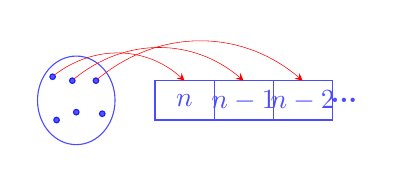
\begin{tikzpicture}
		\draw[blue!70!white] (0.5,0.5) ellipse (14pt and 16pt);
		\fill[draw=\ldraw, fill opacity=0.75, blue!90!white] (0.25, 0.25) circle (1pt) (0.20, 0.80) circle (1pt) (0.45, 0.75) circle (1pt)
															(0.50, 0.35) circle (1pt) (0.83, 0.33) circle (1pt) (0.75, 0.75) circle (1pt);
		\draw[blue!70!white] (1.5,0.25) rectangle (2.25,0.75) node[pos=.5] {$n$}
							 (2.25,0.25) rectangle (3,0.75) node[pos=.5] {$n-1$}
							 (3,0.25) rectangle (3.75,0.75) node[pos=.5] {$n-2$};
		\draw [red, very thin, ->] (0.22, 0.82) to [bend left=40] (1.875, 0.75);
		\draw [red, very thin, ->] (0.47, 0.77) to [bend left=40] (2.625, 0.75);
		\draw [red, very thin, ->] (0.77, 0.77) to [bend left=40] (3.375, 0.75);
		\node {};
		\draw (3.9,0.5) node[blue!70!white] {$\boldsymbol{...}$};
	\end{tikzpicture}
\end{minipage}%
\begin{minipage}{0.35\linewidth}
	\vspace{3mm}
	\bcentering{n(n-1)(n-2)...(1)=n!}
\end{minipage}%
}

\examplebox{
You're given the set of letters \{A,B,C,D,E\}. What is the probability that in a random five-letter string (each letter appears exactly once and all such
strings are equally likely) the letters A and B are next to each other?\\
\vspace{1mm}
By fixing the pair "AB" we have 4 elements in the set $\then$ Probability = $\frac{4!\times2}{5!}$
}

\sectionbox{\subsubsection{Combinations}\topline
Let ${n \choose k}$ be the total number of \textbf{unique combinations} of $k$ elements from a set of $n$ elements. To obtain this number we can proceed with:\\
\vspace{1mm}
{\centering
$\underbrace{n(n-1)(n-2)...(n-k+1)}_{k\text{ elements}}=\frac{n!}{(n-k)!}$
\\}
\vspace{1mm}
But by doing so, we are counting repeated subsets such as \{A,B,C,D,E\} and \{B,A,C,D,E\}. So, in order to avoid permutations, we divide by $k!$, therefore:
\bcentering{\tbinom{n}{k}=\frac{n!}{k!(n-k)!}}
}

\sectionbox{\subsubsection{Binomial Theorem}\topline
Notice that in the expansion of:
\centerexpr{$(x+y)^n = \underbrace{(x+y)...(x+y)}_{k\text{ factors}}\underbrace{(x+y)...(x+y)}_{n-k \text{ factors}}$}
there are ${n \choose k}$ elements of the form $x^{k}y^{n-k}$. So, in order to account for the grouped sum of all terms:
\bcentering{(x+y)^n = \sum_{k=0}^{n}\tbinom{n}{k}x^{k}y^{n-k} \qed}
}

\sectionbox{\subsubsection{Another approach for the number of subsets}\topline
Notice that: $\sum_{k=0}^{n}{n \choose k}= {n \choose 0} + {n \choose 1} + ... + {n \choose n} = \text{Number of subsets}$, therefore:
\bcentering{\sum_{k=0}^{n}\tbinom{n}{k}=(1+1)^n=2^n}
}

\sectionbox{\subsubsection{Partitions}\topline
We have $n$ elements and we need to form $r$ groups of $n_i$ elements each such that $\sum n_i = n$.\\
Let the following expression represent that idea:
\centerexpr{$M=\tbinom{n}{n_1, n_2, ..., n_r}$}
Notice that if we first take $n_1$ elements, we'd have $(n-n_1)$ from which we can take $n_2$, and so on...
\begin{align*}
	M &= \tbinom{n}{n_1} \tbinom{n-n_1}{n_2} \tbinom{n-n_1-n_2}{n_3}...\tbinom{n-n_1-...-n_{r-1}}{n_r} \\
	M &= \frac{n!}{n_{1}!(n-n_1)!} \cdot \frac{(n-n_1)!}{n_2!(n-n_{1}-n_{2})!} \cdot ... \cdot \frac{(n - n_1 - n_2 - ... - n_{r-1})!}{n_r!(0!)}
\end{align*}
Then
\bcentering{\tbinom{n}{n_1, n_2, ..., n_r}=\frac{n!}{n_{1}!n_{2}!...n_{r}!} \qed}
}

\examplebox{\subsubsection{Chess Tournament \& Item Distribution}\topline
Consider the following two problems:
\vspace{0.5mm}
\begin{itemize}
	\item \textbf{Chess tournament: } There are 10 competitors: 4 Russian, 3 from US, 2 from UK, 1 from Brazil. If the tournament result lists just the nationalities 
			of the players, how many outcomes are possible?
	\item \textbf{Distribution of items: } 10 items are to be distributed to 4 people such that they receive 4, 3, 2, 1 items, respectively, how many outcomes are possible?
\end{itemize}
\vspace{0.5mm}
The answer for both problems is: $\frac{10!}{4!3!2!1!}$. What is the underlyig logic the relates them? \vspace{1.5mm}\\
Imagine that the item distribution is executed in the following fashion: Person 1 is placed in front of the items (arranged in a row), then he/she is assigned
items 1,2,3,4 or 1,2,4,3 or ... (i.e. the outcome is the same).\vspace{1.5mm}\\
\begin{minipage}{0.55\linewidth}
	\centering
	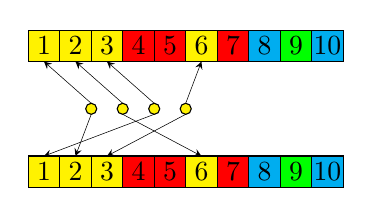
\begin{tikzpicture}
		% Squares
		\draw[fill=yellow] (0,0) rectangle ++(4mm,4mm) node[pos=.5] {1}; 	\draw[fill=yellow] 	(0,-16mm) rectangle ++(4mm,4mm) node[pos=.5] {1};
		\draw[fill=yellow] (4mm,0) rectangle ++(4mm,4mm) node[pos=.5] {2}; 	\draw[fill=yellow] 	(4mm,-16mm) rectangle ++(4mm,4mm) node[pos=.5] {2};
		\draw[fill=yellow] (8mm,0) rectangle ++(4mm,4mm) node[pos=.5] {3}; 	\draw[fill=yellow] 	(8mm,-16mm) rectangle ++(4mm,4mm) node[pos=.5] {3};
		\draw[fill=red] (12mm,0) rectangle ++(4mm,4mm) node[pos=.5] {4};	\draw[fill=red] 	(12mm,-16mm) rectangle ++(4mm,4mm) node[pos=.5] {4};
		\draw[fill=red] (16mm,0) rectangle ++(4mm,4mm) node[pos=.5] {5};	\draw[fill=red] 	(16mm,-16mm) rectangle ++(4mm,4mm) node[pos=.5] {5};
		\draw[fill=yellow] (20mm,0) rectangle ++(4mm,4mm) node[pos=.5] {6};	\draw[fill=yellow] 	(20mm,-16mm) rectangle ++(4mm,4mm) node[pos=.5] {6};
		\draw[fill=red] (24mm,0) rectangle ++(4mm,4mm) node[pos=.5] {7};	\draw[fill=red] 	(24mm,-16mm) rectangle ++(4mm,4mm) node[pos=.5] {7};
		\draw[fill=cyan] (28mm,0) rectangle ++(4mm,4mm) node[pos=.5] {8};	\draw[fill=cyan] 	(28mm,-16mm) rectangle ++(4mm,4mm) node[pos=.5] {8};
		\draw[fill=green] (32mm,0) rectangle ++(4mm,4mm) node[pos=.5] {9};	\draw[fill=green] 	(32mm,-16mm) rectangle ++(4mm,4mm) node[pos=.5] {9};
		\draw[fill=cyan] (36mm,0) rectangle ++(4mm,4mm) node[pos=.5] {10}; 	\draw[fill=cyan] 	(36mm,-16mm) rectangle ++(4mm,4mm) node[pos=.5] {10};
		% Yellow balls
		\foreach \i in {0,...,3} {
			\draw[black, fill=yellow] (\the\numexpr 8 + \i*4\relax mm, -6mm) circle (2pt);
		}
		% Arrows
		\draw [black, very thin, ->] (8 mm, -5.3mm) to (2mm, 0mm); \draw [black, very thin, ->] (8 mm, -6.7mm) to (6mm, -12mm);
		\draw [black, very thin, ->] (12 mm, -5.3mm) to (6mm, 0mm); \draw [black, very thin, ->] (12 mm, -6.7mm) to (22mm, -12mm);
		\draw [black, very thin, ->] (16 mm, -5.3mm) to (10mm, 0mm); \draw [black, very thin, ->] (16 mm, -6.7mm) to (2mm, -12mm);
		\draw [black, very thin, ->] (20 mm, -5.3mm) to (22mm, 0mm); \draw [black, very thin, ->] (20 mm, -6.7mm) to (10mm, -12mm);
	\end{tikzpicture}
\end{minipage}
\begin{minipage}{0.40\linewidth}
	Now imagine that the yellow balls represent the four russian players and also the four item assignments to person 1, for the chess and item distribution problems respectively.\vspace{1.5mm}\\
	It doesn't matter which yellow ball is assigned first, different permutations for this particular arrangement/outcome are counted as one.
\end{minipage}
}

\examplebox{\subsubsection{Ace distribution problem}\topline
There's a 52-card deck, dealt (fairly) to four players. Find the probability that each player gets an ace.\\
\vspace{1.5mm}
\begin{minipage}{0.35\linewidth}
	\centering
	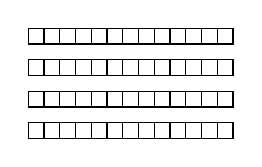
\begin{tikzpicture}[scale=0.5] % scale for better viewing
		\foreach \i in {0,...,3} {
			\foreach \j in {0,...,12} {
			\draw[black, thin] (4mm*\j, -\i*8mm) rectangle ++(4mm,4mm);
			}
		}
	\end{tikzpicture} 
\end{minipage}
\begin{minipage}{0.62\linewidth}
	\textbf{Combinatorial Approach:} There are $4!$ ways of distributing the aces. For the remaining cards, there are $\frac{48!}{(12!)^{4}}$ possibilities.
		$|\Omega|=\frac{52!}{(13!)^{4}} \then P(\text{Event})=4!\frac{48!}{(12!)^{4}}/\frac{52!}{(13!)^{4}}$
	\vspace{2mm}\\
	\textbf{Conditional Probability Approach:} After we randomly deliver the first ace to one of the players,
		there are 39 slots out of the remaining 51 which do not correspond to the player that got an ace.\\
		Following this logic $\then P(\text{Event})=(\frac{52}{52})(\frac{39}{51})(\frac{26}{50})(\frac{13}{49})$ 
\end{minipage}
}

\sectionbox{\subsubsection{Multinomial Theorem}\topline
The expansion of $(x_1 + x_2 + ... + x_r)^n$ will produce $r^n$ elements of the form $x_{1}^{n_1}x_{2}^{n_2}...x_{r}^{n_r}$ such that $\sum n_i = n$. 
\vspace{1.5mm}\\
Some of these elements are identical and can be grouped exactly as those from the expansion in the Binomial Theorem.
\vspace{1.5mm}\\
This is equivalent to listing all the possible divisions of $n$ distinct elements into $r$ distinct groups of sizes $n_1, n_2, . . . , n_r$,
but there are more than one such combinations that add up to $n$, so:
\bcentering{(x_{1} + x_{2} + ... + x_{r})^n = \sum_{\substack{(n_1,...,n_r): \\ n_1+...+n_r=n}} \tbinom{n}{n_1,n_2,...,n_r} x_{_1}^{n_1} x_{_2}^{n_2} ... x_{_r}^{n_r}}
}

\examplebox{\subsubsection{Counting committees}\topline
We start with a pool $n$ of people. A chaired committee consists of $k \geq 1$ members, out of whom one member is designated as the chairperson. Then, the total number of possible chaired committees
of any size is:\; $\sum_{k=1}^{n}k{n \choose k}$. On the other hand, we can also get to the result by first selecting a chairperson and then the committee: $n$ possibilities for the chairperson,
$2^{n-1}$ possible subsets of $n-1$ (the empty set + the chairperson would make a $1$-man committee), so $\sum_{k=1}^{n}k{n \choose k} = n2^{n-1}$.
}

\sectionbox{\subsubsection{Binomial Probabilities}\topline
Consider an experiment with a binary outcome (e.g. success/failure, yes/no, heads/tails, 0/1).\\
Let $p$ be the probability of success $\then$ The probability of $k$ successes in $n$ \textbf{independent} trials is:
\bcentering{P(k \text{ successes})=\tbinom{n}{k}p^k(1-p)^{n-k}}
Also, notice that $\sum_{k=0}^{n} \tbinom{n}{k}p^k(1-p)^{n-k} = 1$
}

\examplebox{\subsubsection{Conditional coin tossing}\topline
Find the probability that the 6th toss out of a total of 10 tosses is Heads, given that there are exactly 2 Heads out of the 10 tosses.\\
\vspace{1.5mm}
\textbf{Binomial Probabilistic Approach:}\\
$P(B)=\tbinom{10}{2}p^2(1-p)^8, \; P(A \cap B)=P(H_{6}\cap \text{One more }H)=p\tbinom{9}{1}p(1-p)^8$\\
$\then P(A|B)=\tbinom{9}{1}/\tbinom{10}{2}$\\
\vspace{1.5mm}
\textbf{Conditional Uniformity Approach:}
\begin{itemize}
	\item Consider $\Omega$ as the set of all possible sequences of 10-tosses.
	\item Let $B$ be the subset that includes exactly 2 heads. There are $\tbinom{10}{2}$ such elements, all with probability $p^2(1-p)^8$.
	\item Let $A$ be the subset that includes $H_6$. Since $H_6$ is fixed, there are $\tbinom{9}{1}$ ways for $A \cap B$ to occur.
		And because these elements are included in $B$, they have probability $p^2(1-p)^8$.
	\item $\then P(A|B)=\tbinom{9}{1}/\tbinom{10}{2}$
\end{itemize}
}


\titlebox{\section{Discrete Random Variables}}

\subsection{Random Variables}

\sectionbox{\subsubsection{Random Variable}\topline
\vspace{0.75mm}
\begin{minipage}{0.52\linewidth}
	\centering
	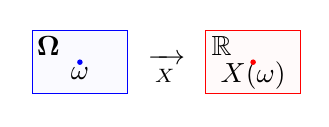
\begin{tikzpicture}
		\draw[thin, blue, fill=blue!2!white] (0mm,0mm) rectangle ++(12mm,8mm);
		\node at (2mm, 6mm) {$ \boldsymbol{\Omega} $}; \node at (6mm, 2.5mm) {$ \omega $}; \fill[blue] (6mm, 4mm) circle (1pt);
		\node at (17mm, 3mm) {$ \xrightarrow[X]{} $};
		\draw[thin, red, fill=red!2!white] (22mm,0mm) rectangle ++(12mm,8mm);
		\node at (24mm, 6mm) {$ \mathbb{R} $}; \node at (28mm, 2.25mm) {$ X(\omega) $}; \fill[red] (28mm, 4mm) circle (1pt);
	\end{tikzpicture}
\end{minipage}
{\centering\fbox{%
\begin{minipage}{0.40\linewidth}
\textbf{Simple Definition:}\vspace{0.5mm}\\
A random variable $X(\omega)$ or simply $X$ is a function defined on the sample space $\Omega$ that associates its outcomes to $\mathbb{R}$.
\centerexpr{$ X\colon \Omega \to \mathbb{R}$}
\end{minipage}}\\}%
\vspace{1.25mm}
\begin{itemize}
	\item The term "random variable" can be misleading since it's a function rather than a variable.
	\item More formally, it is a measurable function \;$X\colon \Omega \to R$\;\, from $\Omega$ into a measurable space $R$.
	\item The outcome itself can be thought of as a random variable \\
		$\then \Omega=R, X(\omega)=\omega \rightarrow$ Identity function.
\end{itemize}
}

\sectionbox{\subsubsection{Notation}\topline
\begin{itemize}
	\item $X(\omega)$ or simply $X$ is a random variable, a function defined on the domain $\Omega$ with range in $\mathbb{R}$.
	\item $x$ is an unspecified value of $X \then x$ is a real variable such that $x\in\mathbb{R}$.
	\item $\{X=a\} \Blue{\iff} \{\omega:X(\omega) = a\}$, both imply an \textbf{event} in which $X$ takes the particular value $a$.
	\item $\{X=a\} = \{\omega:X(\omega) = a\}$ only if the outcome itself is the random variable.
	\item $\{X=x\}$ is an unspecified (variable) event in which $X$ takes the unspecified value $x$.
	\item $P\boldsymbol{(}\{X=x\}\boldsymbol{)}$ is the probability of that unspecified event $\rightarrow$ We will write $P(X=x)$ for short.\\
	$\then P\boldsymbol{(}\{\omega:X(\omega) = 3\}\boldsymbol{)} \Blue{\iff} P(X=3)$
\end{itemize}
}

\sectionbox{\subsubsection{Function of Random Variables}\topline
{\centering\fbox{%
\begin{minipage}{0.67\linewidth}
	Let $X$ be a random variable with values in $S \then X:\Omega \to S \subseteq \mathbb{R}$.\\
	Let $g$ be a function defined on $S$ that maps into $T \then g:S \to T$.\\
	$\then$ $g(X)$ depends on $X \then g(X)$ depends on the values in $\Omega$.\\
	$\then Y=g(X)$ is a random variable with values in $T. \qed$
\end{minipage}}\\}%
\par\vspace{1.5mm}
{\centering\fbox{%
\begin{minipage}{0.67\linewidth}
	Let $X$ and $Y$ be random variables.\\
	Let $g(X,Y)$ be a function of the random variables $X$ and $Y$.\\
	$\forall x,y:(X=x \land Y=y) \then g(X,Y)=g(x,y)$.\\
	However, the converse is not necessarily true.
\end{minipage}}\\}%
\vspace{1mm}
Let $X\in\{1,2\} \land Y\in\{3,4\}$ \\
So\quad $X=2 \land Y=3 \then X+Y=5$\\
but\quad $X+Y=5 \then (X=2 \land Y=3) \lor (X=1 \land Y=4) \qed$
}

\sectionbox{\subsubsection{Discrete Random Variable}\topline

{\centering\fbox{%
\begin{minipage}{0.76\linewidth}
A random variable is called discrete if its \textbf{range} is either finite or countably infinite.
\end{minipage}}\\}%
\par\vspace{2mm}
{
\begin{minipage}{0.50\linewidth}
	\centering
	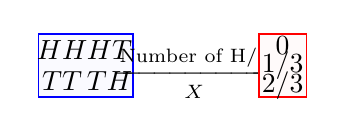
\begin{tikzpicture}
		\draw[thin, blue, fill=blue!2!white] (0mm,0mm) rectangle ++(12mm,8mm);
		\node at (3mm, 6mm) {$ HH $}; \node at (9mm, 6mm) {$ HT $}; \node at (3mm, 2mm) {$ TT $}; \node at (9mm, 2mm) {$ TH $};
		\node at (20mm, 3mm) {$ \xrightarrow[X]{\text{Number of H}/3} $};
		\draw[thin, red, fill=red!2!white] (28mm,0mm) rectangle ++(6mm,8mm);
		\node at (31mm, 6.5mm) {$ 0 $}; \node at (31mm, 4mm) {$ 1/3 $}; \node at (31mm, 1.5mm) {$ 2/3 $};
	\end{tikzpicture}\\
	\[ \text{sgn}(\omega)=
		\begin{cases}
			-1, & \omega<0\\
			0, & \omega=0\\
			1, & \omega>0
		\end{cases}
	\]
\end{minipage}
\begin{minipage}{0.45\linewidth}
	Experiment: 2 tosses of a coin.\\
	Let $X$ be the number of heads divided by 3.\\
	The range is finite: consists of 3 elements.
	\vspace{6mm}\\
	Experiment: Select $\omega : \omega \in [-1,1]$\\
	Let $X=\text{sgn}(\omega)$\\
	The domain is infinite, but the range is finite.
\end{minipage}
}
}

\subsection{Probability Mass Functions \& Expectation}

\sectionbox{\subsubsection{Probability Mass Function}\topline
{\centering\fbox{%
\begin{minipage}{0.70\linewidth}
The function
\centerexpr{$p_{X}(x)=P(X=x)=P({\omega:X(\omega)=x})$}\vspace{0.5mm}
is called the Probability Mass Function (\textbf{PMF}) and assigns a probability to each numerical value of a Discrete Random Variable.
\end{minipage}}\\}%
\vspace{1.5mm}
For simplicity, let $S=\Omega$ be the sample space. The PMF has the following properties:\vspace{0.5mm}
\begin{itemize}
	\item $p_{X}(x) \geq 0, x \in S$
	\item $\displaystyle\sum_{x \in S} p_{X}(x)=1$
	\item $\displaystyle\sum_{x \in A} p_{X}(x)=P(A), \; A\subseteq S$
\end{itemize}
}

\sectionbox{\subsubsection{Graphs of PMF}\topline
{
\begin{minipage}{0.49\linewidth}
	\centering
	Sum of 2 rolls of a tetrahedral die. \vspace{1.5mm}\\
	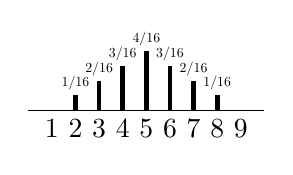
\begin{tikzpicture}[x=3mm, y=30mm] % (each unit on the x axis = 5mm, IDEM for the y axis)
		\draw
		  (0,0) edge[-] (10,0) % the main axis
		  foreach[count=\i from 2] ~ in {1/16,2/16,3/16,4/16,3/16,2/16,1/16}{
			(\i,0) pic[black]{bar={~}{~}} node[below]{$\i$} % 1st ~ = height, 2nd ~ = probability (label) above
		  };
		  \draw (1,0)node[below]{$1$}; \draw (9,0)node[below]{$9$};
	\end{tikzpicture}
\end{minipage}
\begin{minipage}{0.49\linewidth}
	\centering
	PMF of a categorical random variable.\vspace{1.5mm}\\
	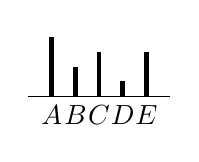
\begin{tikzpicture}[x=3mm, y=30mm] % (each unit on the x axis = 5mm, IDEM for the y axis)
		\draw
		  (0,0) edge[-] (6,0) % the main axis
		  foreach[count=\i from 1] ~ in {4/16,2/16,3/16,1/16,3/16}{
			(\i,0) pic[black]{bar={~}{}}
		  };
		  \draw (1,0)node[below]{$A$}; \draw (2,0)node[below]{$B$}; \draw (3,0)node[below]{$C$}; \draw (4,0)node[below]{$D$}; \draw (5,0)node[below]{$E$};
	\end{tikzpicture}
\end{minipage}
}
\par\vspace{2mm}
{
\begin{minipage}{0.49\linewidth}
	\centering
	$P(X=x)=\frac{1}{2^{x}}$, \quad for $x\in\mathbb{N}$.\vspace{1.5mm}\\
	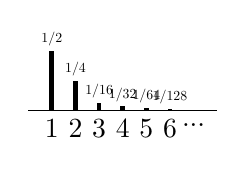
\begin{tikzpicture}[x=3mm, y=15mm] % (each unit on the x axis = 5mm, IDEM for the y axis)
		\draw
		  (0,0) edge[-] (8,0) % the main axis
		  foreach[count=\i from 1] ~ in {1/2,1/4,1/16,1/32,1/64, 1/128}{
			(\i,0) pic[black]{bar={~}{~}} node[below]{$\i$}
		  };
		  \draw (7,-.03)node[below]{$...$};
	\end{tikzpicture}
\end{minipage}
\begin{minipage}{0.49\linewidth}
	\centering
	Discrete Uniform Random Variable.\vspace{1.5mm}\\
	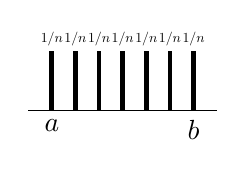
\begin{tikzpicture}[x=3mm, y=30mm] % (each unit on the x axis = 5mm, IDEM for the y axis)
		\draw
		  (0,0) edge[-] (8,0) % the main axis
		  foreach[count=\i from 1] ~ in {4/16,4/16,4/16,4/16,4/16,4/16,4/16}{
			(\i,0) pic[black]{bar={~}{1/n}}
		  };
		  \draw (1,0)node[below]{$a$}; \draw (7,0)node[below]{$b$};
	\end{tikzpicture}
\end{minipage}
}
}

\examplebox{
Consider the experiment of tossing twice a fair tetrahedral die. Let $X$ be the product of the rolls, then:\vspace{1mm}\\
\begin{minipage}{0.70\linewidth}
	\centering
	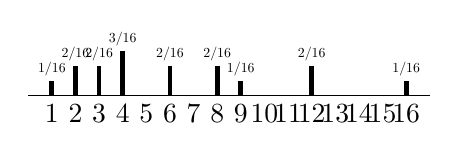
\begin{tikzpicture}[x=3mm, y=30mm] % (each unit on the x axis = 5mm, IDEM for the y axis)
		\draw (0,0) edge[-] (17,0);
		\foreach \i/\j in {1/{1/16},2/{2/16},3/{2/16},4/{3/16},6/{2/16},8/{2/16},9/{1/16},12/{2/16},16/{1/16}} {
			\draw (\i, 0) pic[black]{bar={\j}{\j}};
		}
		\foreach \i in {1,...,16}{
			\draw (\i,0)node[below]{$\i$};
		}
	\end{tikzpicture}
\end{minipage}
\begin{minipage}{0.25\linewidth}
	
	\begin{tabular}{|c|cccc|}
		\hline
		$\times$  & 1 & 2 & 3 & 4 \\
		\hline
		1 & 1 & 2 & 3 & 4 \\ 
		2 & 2 & 4 & 6 & 8 \\
		3 & 3 & 6 & 9 & 12 \\
		4 & 4 & 8 & 12 & 16 \\
		\hline
	\end{tabular}
\end{minipage}\\
\vspace{1mm}
$p_{X}(4)=P(\{1,4\} \cup \{2,2\} \cup \{4,1\})=3/16$\\
$p_{X}(5)=0$
}


\end{multicols*}
\newpage
%#################################################################################################################################
\begin{multicols*}{4}

\sectionbox{\subsubsection{EOQ formula derivation}\topline

Since demand is deterministic, we can get rid of the Stockout Cost concept for now. So,

\begin{align*}
	TRC(Q) &= c_{t}\frac{D}{Q} + c_{e}\frac{Q}{2}
\end{align*}

From the first-order optimal condition (first derivative equals zero), we have

\begin{align*}
	0 &= \diff{}{Q}\left(\frac{c_{t}D}{Q}\right) + \diff{}{Q}\left(\frac{c_{e}Q}{2}\right) \\
	0 &= -\frac{c_{t}D}{Q^2}+\frac{c_{e}}{2} \\
	\Aboxed{Q^{*} &= \sqrt{\frac{2c_{t}D}{c_e}}}
\end{align*}

The $EOQ$ or $Q^*$ gives the minimum $TRC$ under deterministic conditions:

\begin{figure}[H]
	\centering
	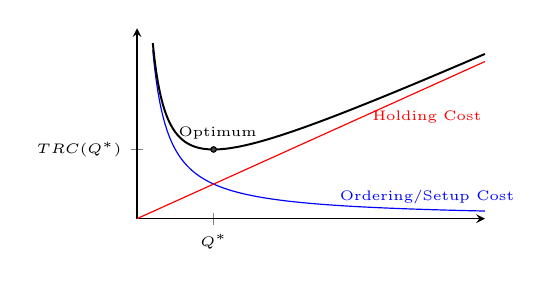
\begin{tikzpicture}
	\tikzmath{\ce=5.5; \ct=400; \D=3000; \xmax=3000; \Qopt=660; \TRCopt=3633.18;}
	\begin{axis}[1Quad, width=6cm, height=4cm, hide scale,
				ymin=0, ymax=10000, xmin=0, xmax=\xmax,
				xtick={\Qopt}, xticklabels={$Q^*$},
				ytick={\TRCopt}, yticklabels={$TRC(Q^*)$},
				restrict y to domain = 0:9500]
		% Functions
		\addplot[blue, line width=0.15mm, domain=0:\xmax]{\ct*(\D/x)};
		\addplot[red, line width=0.15mm, domain=0:\xmax]{\ce*(x/2)};
		\addplot[black, line width=0.25mm, domain=0:\xmax]{\ct*(\D/x) + \ce*(x/2)};
		% Nodes
		\node[circle,draw=black,fill=black!75,inner sep=0pt,minimum size=2pt] at (\Qopt,\TRCopt){};
		% Annotations
		\draw (\Qopt,\TRCopt)node[above, xshift=0.5mm]{\tiny Optimum};
		\draw (2500,250)node[blue, above]{\tiny Ordering/Setup Cost};
		\draw (2500,4500)node[red, above]{\tiny Holding Cost};
	\end{axis}
	\end{tikzpicture}
\end{figure}
}

\sectionbox{\subsubsection{EOQ sawtooth plot}\topline
The optimal policy becomes ordering $Q^*$ units of inventory every $T^*$ units of time.

\begin{figure}[H]
	\centering
	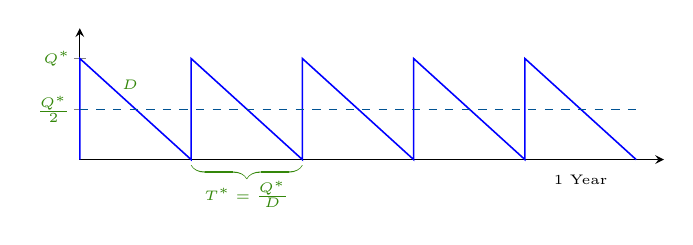
\begin{tikzpicture}
		\tikzmath{\lastx = 5;}
		\begin{axis}[1Quad,width=9cm,height=3.25cm,ymin=0,ymax=1.3,xmin=0,xmax=\lastx + 0.25,
					xtick style={draw=none}, xtick={\lastx-0.5}, xticklabels={1 Year},
					ytick={0.5,1}, yticklabels={,,}
					]
			% Sawtooth
			\draw (0,0) foreach \x in {1,...,\lastx} {-- ++(0,1) -- ++(1,-1)} [blue, line width=0.2mm];
			\draw (0,0.5) -- (\lastx,0.5) [darkblue, dashed, line width=0.02mm];
			\draw [pen colour={annot},decorate,decoration={calligraphic brace,mirror,amplitude=5pt,raise=2pt},xshift=0pt,yshift=0pt]
			(1,0) -- (2,0) node [annot,midway,yshift=-12.5pt, line width=5mm] {\tiny $T^*=\frac{Q^*}{D}$};
			\draw (0,1) node[annot, left]{\tiny $Q^*$};
			\draw (0,0.5) node[annot, left]{\tiny $\frac{Q^*}{2}$};
			\draw (0.45,0.6) node[annot, above]{\tiny $D$};
		\end{axis}
		\end{tikzpicture}
\end{figure}

Notice that the total consumption of the last order may take place after the 1 year (unit time) period.

}



\subsection{Mathematical Functions}
\sectionbox{\subsubsection{Linear Functions}\topline

\[ f(x) = mx+b \]

\textbf{Cost functions: } $f(\text{Level of Activity})=\text{Fixed Cost} + \text{Variable Cost}(\text{Level of Activity})$

\begin{figure}[H]
	\centering
	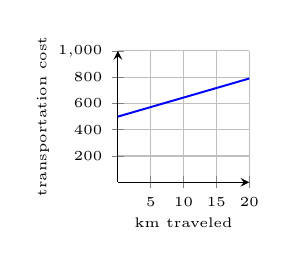
\begin{tikzpicture}
		\begin{axis}[
					1Quad,width=3.25cm,height=3.25cm,
					ymin=0, ymax=1000, grid=both,
					xlabel = {km traveled}, x label style={at={(axis description cs:0.5,-0.2)}, anchor=north},
					ylabel = {transportation cost}, y label style={at={(axis description cs:-0.45,.5)},rotate=90,anchor=south},
					%ticklabel style = font={\fontsize{1}{1}\selectfont},
					]
			\addplot[blue, line width=0.25mm, domain=0:20]{500+14.5*x};
		\end{axis}
	\end{tikzpicture}
	\hspace{0.25cm}
	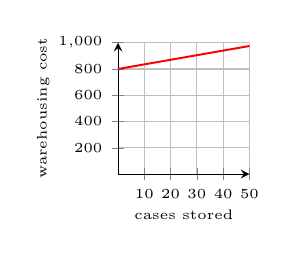
\begin{tikzpicture}
		\begin{axis}[1Quad,width=3.25cm,height=3.25cm,
					ymin=0,ymax=1000,
					xtick={10,20,30,40,50}, grid=both,
					xlabel = {cases stored}, x label style={at={(axis description cs:0.5,-0.2)}, anchor=north},
					ylabel = {warehousing cost}, y label style={at={(axis description cs:-0.45,.5)},rotate=90,anchor=south},
					]
			\addplot[red, line width=0.25mm, domain=0:50]{800+3.5*x};
		\end{axis}
	\end{tikzpicture}
\end{figure}

\textbf{Linear Regressions}

fig
}

\sectionbox{\subsubsection{Quadratic Functions}\topline

\[ f(x) = ax^2+bx+c \]

\textbf{Profit: }


\begin{figure}[H]
	\begin{minipage}{0.5\linewidth}\centering
		
		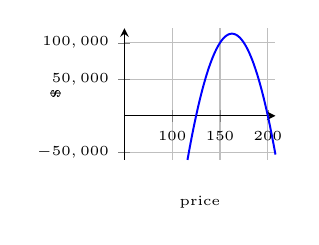
\begin{tikzpicture}
			\begin{axis}[
						1Quad,width=3.5cm,height=3.25cm,
						xmin = 50,
						ymin=-60000, ymax=120000, grid=both,
						scaled y ticks = false, scaled x ticks = false, 
						y tick label style={/pgf/number format/.cd, fixed, fixed zerofill, int detect,1000 sep={,},precision=2},
						x tick label style={/pgf/number format/.cd, fixed, fixed zerofill, int detect, 1000 sep={},precision=2},
						xlabel = {price}, x label style={at={(axis description cs:0.5,-0.2)}, anchor=north},
						ylabel = {\$}, y label style={at={(axis description cs:-0.35,.5)},rotate=90,anchor=south}
						]
				\addplot[blue, line width=0.25mm, domain=116:208]{-80*x^2 + 26000*x - 2000000};
			\end{axis}
		\end{tikzpicture}
	\end{minipage}
	\begin{minipage}{0.5\linewidth}\centering
		\tiny{
		\begin{align*}
			&V(p) = 20,000 - 80p \\
			&R(p) = (20,000 - 80p)p \\
			&C(p) = 500,000 + 75(20,000 - 80p) \\
			&P(p) = R(p) - C(p)
		\end{align*}}
		\vfill
	\end{minipage}
\end{figure}


\textbf{Parcel trucking}

\begin{figure}[H]
	\begin{minipage}{0.5\linewidth}\centering
		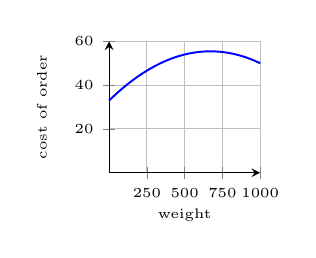
\begin{tikzpicture}
			\begin{axis}[
						1Quad,width=3.5cm,height=3.25cm,
						ymin=-0, ymax=60, grid=both,
						scaled y ticks = false, scaled x ticks = false,
						xtick={250, 500, 750, 1000},
						y tick label style={/pgf/number format/.cd, fixed, fixed zerofill, int detect,1000 sep={,},precision=2},
						x tick label style={/pgf/number format/.cd, fixed, fixed zerofill, int detect, 1000 sep={},precision=2},
						xlabel = {weight}, x label style={at={(axis description cs:0.5,-0.2)}, anchor=north},
						ylabel = {cost of order}, y label style={at={(axis description cs:-0.35,.5)},rotate=90,anchor=south}
						]
				\addplot[blue, line width=0.25mm, domain=0:1000]{33 + 0.067*x - 0.00005*x^2};
			\end{axis}
		\end{tikzpicture}
	\end{minipage}
	\begin{minipage}{0.5\linewidth}\centering
		\tiny{
		\begin{align*}
			&f(w) = 33 + 0.067w - 0.00005w^2
		\end{align*}}
		\vfill
	\end{minipage}
\end{figure}

}

\end{multicols*}

\newpage


\begin{multicols*}{2}
\titlebox{\section{Proofs:}}
\subsection{Inclusion-Exclusion Principle} \label{Inclusion-Exclusion Principle}
\vspace{1.5mm}
Consider the cases for $n=3$ and $n=4$:
\begin{flalign*}
	P(A_1\cup A_2\cup A_3)= & \;\;\;\; P(A_1)+P(A_2) +P(A_3) & \\ % Last & is for full left alignment (just this first line for the whole flalign environment)
	& -\underbrace{P(A_1\cap A_{2})}_{1<2} -\underbrace{P(A_1\cap A_{3})}_{1<3} -\underbrace{P(A_2\cap A_{3})}_{2<3} \\
	& +\underbrace{P(A_1\cap A_{2}\cap A_{3})}_{1<2<3}
\end{flalign*}
\begin{flalign*}
	P(A_1\cup A_2\cup A_3\cup A_4)= & \;\;\;\; P(A_1)+P(A_2) +P(A_3)+P(A_4) &\\
	&
	-\underbrace{P(A_{1}\cap A_{2})}_{1<2}
	-\underbrace{P(A_{1}\cap A_{3})}_{1<3}
	-\underbrace{P(A_{1}\cap A_{4})}_{1<4}
	-\underbrace{P(A_{2}\cap A_{3})}_{2<3}
	-\underbrace{P(A_{2}\cap A_{4})}_{2<4}
	-\underbrace{P(A_{3}\cap A_{4})}_{3<4}
	\\
	&
	+\underbrace{P(A_{1}\cap A_{2}\cap A_{3})}_{1<2<3}
	+\underbrace{P(A_{1}\cap A_{2}\cap A_{4})}_{1<2<4}
	+\underbrace{P(A_{1}\cap A_{3}\cap A_{4})}_{1<3<4}
	+\underbrace{P(A_{2}\cap A_{3}\cap A_{4})}_{2<3<4}
	\\
	&
	-\underbrace{P(A_1\cap A_{2}\cap A_{3}\cap A_4)}_{1<2<3<4}.
\end{flalign*} 
We argue that we have a general pattern:
\begin{flalign*}
	P\left( \bigcup_{i=1}^{n} A_i\right) = &-(-1)^1 \sum_{1 \leq i \leq n} P(A_{i}) &\\
	& -(-1)^2 \sum_{1\leq i_{_1}<i_{_2} \leq n} P(A_{i_1} \cap A_{i_2}) \\
	& -(-1)^3 \sum_{1\leq i_{_1}<i_{_2}<i_{_3} \leq n} P(A_{i_1} \cap A_{i_2} \cap A_{i_3}) \\
	& -(-1)^4 \sum_{1\leq i_{_1}<i_{_2}<i_{_3}<i_{_4} \leq n} P(A_{i_1} \cap A_{i_2} \cap A_{i_3} \cap A_{i_4}) \\
	& \quad\quad\quad\vdots \\
	& -(-1)^n \, P(A_{1}\cap A_{2}\cap A_{3}\cap A_{4}\cap... \cap A_{n}) \\
	\Aboxed{P\left( \bigcup_{i=1}^{n} A_i\right) = &-\sum_{k=1}^{n} (-1)^k \sum_{1 \leq i_{_1} < ... < i_{_k} \leq n} P \left( \, \bigcap_{j=1}^{k} A_{i_j} \right) }
\end{flalign*}
\textbf{Proof by Induction:}\\
Suppose the pattern is true for $n$, we need to show it works for $n+1$. First, consider $n=2$ and apply distributivity:
\begin{flalign*}
	P(A_{1} \cup A_{2} \cup ... \cup A_{n} \cup A_{n+1}) &= P\big( (A_{1} \cup A_{2} \cup ... \cup A_{n}) \cup A_{n+1} \big) &\\
	& = P(A_{1} \cup A_{2} \cup ... \cup A_{n}) + P(A_{n+1}) - P\big( (A_{1} \cup A_{2} \cup ... \cup A_{n}) \cap A_{n+1} \big) \\
	& = \underbrace{P(A_{1} \cup A_{2} \cup ... \cup A_{n})}_{n \:\: \text{unions}} + P(A_{n+1}) - 
	\underbrace{P\big( (A_{1} \cap A_{n+1}) \cup (A_{2} \cap A_{n+1}) \cup ... \cup (A_{n} \cap A_{n+1}) \big)}_{n \:\: \text{unions}}
\end{flalign*}
The first and the last terms are n-unions, for which we assumed the formula to hold. Therefore:
\begin{flalign}
	P(A_{1} \cup A_{2} \cup ... \cup A_{n} \cup A_{n+1}) = & \textcolor{blue}{ \; -(-1)^1 \sum_{1 \leq i \leq n} P(A_{i})} &\\
	& \textcolor{red}{-(-1)^2 \sum_{1\leq i_{_1}<i_{_2} \leq n} P(A_{i_1} \cap A_{i_2})} \\
	& \textcolor{green!60!black}{-(-1)^3 \sum_{1\leq i_{_1}<i_{_2}<i_{_3} \leq n} P(A_{i_1} \cap A_{i_2} \cap A_{i_3})} \\
	& - ... \textcolor{orange!70!black}{-(-1)^n \, P(A_{1}\cap A_{2}\cap A_{3}\cap A_{4}\cap... \cap A_{n})} \\
	& + \textcolor{blue}{P(A_{n+1})} \\
	& + \textcolor{red}{(-1)^1 \sum_{1 \leq i \leq n} P(A_{i} \cap A_{n+1})} \\
	& + \textcolor{green!60!black}{(-1)^2 \sum_{1\leq i_{_1}<i_{_2} \leq n} P(A_{i_1} \cap A_{i_2} \cap A_{n+1})} \\
	& + ... \textcolor{orange!70!black}{+(-1)^{n-1} \sum_{1\leq i_{_1}<i_{_2}<...<i_{n-1}\leq n} P(A_{i_1} \cap A_{i_2} \cap ... \cap A_{i_{n-1}} \cap A_{n+1})} \\
	& + (-1)^n \, P(A_{1}\cap A_{2}\cap A_{3}\cap A_{4}\cap... \cap A_{n} \cap A_{n+1})
\end{flalign}
Here (1) and (5) account for all the probabilities of single events from $1$ to $n + 1$. (2) includes all the two-
intersection probabilities from $1$ to $n$, and (6) all the two-intersection probabilities where the higher index equals
$n + 1$. These two sums thus account for all possible two-intersection probabilities from $1$ to $n + 1$. Similarly,
(3) includes all three-intersection probabilities from $1$ to $n$, and (7) those with highest index equal to $n + 1$.
Together they include all three-intersection probabilities from $1$ to $n + 1$.\\

\begin{minipage}{3cm}
\tikzmath{\a = 0.5; \b = 0.05;}
\begin{tikzpicture}[scale=0.75]
	\begin{scope}[draw=black, fill opacity=0.75]
		\fill[Emerald] (0, 0) rectangle (\a, \a); \draw (0,0) node[above, xshift=2mm, yshift=3.5mm]{\tiny $A_{_1}$};
		\fill[Emerald] (\a + \b, 0) rectangle (2*\a + \b, \a); \draw (\a + \b,0) node[above, xshift=2mm, yshift=3.5mm]{\tiny $A_{_2}$};
		\fill[Emerald] (2*\a + 2*\b, 0) rectangle (3*\a + 2*\b, \a); \draw (2*\a + 2*\b,0) node[above, xshift=2mm, yshift=3.5mm]{\tiny $A_{_3}$};
		\fill[Emerald] (3*\a + 3*\b, 0) rectangle (4*\a + 3*\b, \a); \draw (3*\a + 3*\b,0) node[above, xshift=2mm, yshift=3.5mm]{\tiny $A_{_4}$};
																	\draw (3*\a + 3*\b,0) node[above, xshift=2mm, yshift=0mm]{\tiny $i_{4}$};
		\fill[white] (4*\a + 4*\b, 0) rectangle (5*\a + 4*\b, \a); \draw (4*\a + 4*\b,0) node[above, xshift=2mm, yshift=3.5mm]{\tiny $A_{_5}$};
		\fill[Emerald] (5*\a + 5*\b, 0) rectangle (6*\a + 5*\b, \a); \draw (5*\a + 5*\b,0) node[above, xshift=2mm, yshift=3.5mm]{\tiny $A_{_6}$};

		\fill[Emerald] (0, -\a - \b) rectangle (\a, 0- \b);
		\fill[Emerald] (\a + \b, -\a- \b) rectangle (2*\a + \b, 0- \b);
		\fill[Emerald] (2*\a + 2*\b, -\a- \b) rectangle (3*\a + 2*\b, 0- \b);
		\fill[white] (3*\a + 3*\b, -\a- \b) rectangle (4*\a + 3*\b, 0- \b);
		\fill[Emerald] (4*\a + 4*\b, -\a- \b) rectangle (5*\a + 4*\b, 0- \b); \draw (4*\a + 4*\b, -\a- \b) node[above, xshift=2mm, yshift=0mm]{\tiny $i_{4}$};
		\fill[Emerald] (5*\a + 5*\b, -\a- \b) rectangle (6*\a + 5*\b, 0- \b);

		\fill[Emerald] (0, -2*\a - 2*\b) rectangle (\a, -\a - 2*\b);
		\fill[Emerald] (\a + \b, -2*\a- 2*\b) rectangle (2*\a + \b, -\a - 2*\b);
		\fill[white] (2*\a + 2*\b, -2*\a- 2*\b) rectangle (3*\a + 2*\b, -\a - 2*\b);
		\fill[Emerald] (3*\a + 3*\b, -2*\a- 2*\b) rectangle (4*\a + 3*\b, -\a - 2*\b);
		\fill[Emerald] (4*\a + 4*\b, -2*\a- 2*\b) rectangle (5*\a + 4*\b, -\a - 2*\b); \draw (4*\a + 4*\b, -2*\a- 2*\b) node[above, xshift=2mm, yshift=0mm]{\tiny $i_{4}$};
		\fill[Emerald] (5*\a + 5*\b, -2*\a- 2*\b) rectangle (6*\a + 5*\b, -\a - 2*\b);

		\fill[Emerald] (0, -3*\a - 3*\b) rectangle (\a, -2*\a - 3*\b);
		\fill[white] (\a + \b, -3*\a- 3*\b) rectangle (2*\a + \b, -2*\a - 3*\b);
		\fill[Emerald] (2*\a + 2*\b, -3*\a- 3*\b) rectangle (3*\a + 2*\b, -2*\a - 3*\b);
		\fill[Emerald] (3*\a + 3*\b, -3*\a- 3*\b) rectangle (4*\a + 3*\b, -2*\a - 3*\b);
		\fill[Emerald] (4*\a + 4*\b, -3*\a- 3*\b) rectangle (5*\a + 4*\b, -2*\a - 3*\b); \draw (4*\a + 4*\b, -3*\a- 3*\b) node[above, xshift=2mm, yshift=0mm]{\tiny $i_{4}$};
		\fill[Emerald] (5*\a + 5*\b, -3*\a- 3*\b) rectangle (6*\a + 5*\b, -2*\a - 3*\b);

		\fill[white] (0, -4*\a - 4*\b) rectangle (\a, -3*\a - 4*\b);
		\fill[Emerald] (\a + \b, -4*\a- 4*\b) rectangle (2*\a + \b, -3*\a - 4*\b);
		\fill[Emerald] (2*\a + 2*\b, -4*\a- 4*\b) rectangle (3*\a + 2*\b, -3*\a - 4*\b);
		\fill[Emerald] (3*\a + 3*\b, -4*\a- 4*\b) rectangle (4*\a + 3*\b, -3*\a - 4*\b);
		\fill[Emerald] (4*\a + 4*\b, -4*\a- 4*\b) rectangle (5*\a + 4*\b, -3*\a - 4*\b); \draw (4*\a + 4*\b, -4*\a- 4*\b) node[above, xshift=2mm, yshift=0mm]{\tiny $i_{4}$};
		\fill[Emerald] (5*\a + 5*\b, -4*\a- 4*\b) rectangle (6*\a + 5*\b, -3*\a - 4*\b);
	\end{scope}
\end{tikzpicture}
\end{minipage}
\begin{minipage}{13cm}
	This continues until (4) and (8), which together give all n-intersection probabilities from $1$ to $n + 1$. To see why this is true, let's consider the case for $n=5$ (i.e. we
	would prove that the formula applies for $n=6$). It could be the case that $A_{i_{n-1}} = A_{i_4} = A_{5}$ (see the figure), so equation (8) would give all the combinations on the figure
	(emerald squares), and equation number (4) would give the missing intersection: $A_{1} \cap A_{2} \cap A_{3} \cap A_{4} \cap A_{5}$.
\end{minipage}
\vspace{2mm}
\\
Finally, we write the last term (9) and, therefore, we observe that:
\begin{flalign*}
	P\left( \bigcup_{i=1}^{n+1} A_i\right) = &-(-1)^1 \sum_{1 \leq i \leq n+1} P(A_{i}) &\\
	& -(-1)^2 \sum_{1\leq i_{_1}<i_{_2} \leq n+1} P(A_{i_1} \cap A_{i_2}) \\
	& -(-1)^3 \sum_{1\leq i_{_1}<i_{_2}<i_{_3} \leq n+1} P(A_{i_1} \cap A_{i_2} \cap A_{i_3}) \\
	& - ... -(-1)^n \sum_{1\leq i_{_1}<i_{_2} <...<i_{_n} \leq n+1} P(A_{i_1} \cap A_{i_2} \cap ... \cap A_{i_n}) \\
	& -(-1)^{n+1} \, P(A_{1}\cap A_{2}\cap A_{3}\cap A_{4}\cap... \cap A_{n+1})
\end{flalign*}
We have proven that the expression works for $n+1 \qed$

\end{multicols*}

\newpage

\begin{multicols*}{2}
\titlebox{\section{References:}} \vspace{1.75mm}
\subsection{Books}
2008 - Introduction to Probability (2nd ed.) - Dimitri P. Bertsekas \& John N. Tsitsiklis \\
\href{https://stats.libretexts.org/Bookshelves/Probability_Theory/Probability_Mathematical_Statistics_and_Stochastic_Processes_(Siegrist)}
{2021 - Probability, Mathematical Statistics, and Stochastic Processes - Kyle Siegrist}
\subsection{MIT OpenCourseWare}
\url{https://www.youtube.com/playlist?list=PLUl4u3cNGP60A3XMwZ5sep719_nh95qOe}
\subsection{Links}
\textbf{Inclusion-Exclusion Principle}\\
\url{https://math.stackexchange.com/questions/2587979/generalized-formula-for-the-probability-of-the-union-of-n-events-occurring}\\
\url{https://people.maths.bris.ac.uk/~mb13434/incl_excl_n.pdf}\\
\textbf{Event Independence}\\
\url{https://math.stackexchange.com/questions/1832686/probability-are-disjoint-events-independent}\\
\textbf{Random Variables}\\
\url{https://en.wikipedia.org/wiki/Random_variable}\\
\href{https://stats.libretexts.org/Bookshelves/Probability_Theory/Probability_Mathematical_Statistics_and_Stochastic_Processes_(Siegrist)/02%3A_Probability_Spaces/2.02%3A_Events_and_Random_Variables#Random_Variables}{Siegrist: Random Variables}
\end{multicols*}

\end{document}